% !TeX program = xelatex
% !TeX TXS-program:compile = txs:///xelatex/[--shell-escape]
%%%%%%%%%%%%%%%%%%%%%%%%%%%%%%%%%%%%%%%%%%%%%%%%%%%%%%%%%%%%%%%%%%%%%%%%
% Plantilla TFG/TFM
% Escuela Politécnica Superior de la Universidad de Alicante
% Realizado por: Jose Manuel Requena Plens
% Contacto: info@jmrplens.com / Telegram:@jmrplens
%%%%%%%%%%%%%%%%%%%%%%%%%%%%%%%%%%%%%%%%%%%%%%%%%%%%%%%%%%%%%%%%%%%%%%%%

% Elige si deseas optimizar la ejecución del proyecto almacenando las figuras generadas con TikZ y PGF en una carpeta (archivos/figuras-procesadas).
% 1 - Si, 2 - No
\def\OptimizaTikZ{1}

% Archivo .TEX que incluye todas las configuraciones del documento y los paquetes. Añade todo aquello que necesites utilizar en el documento en este archivo.
% En él se encuentra la configuración de los márgenes, establecidos según las directrices de estilo de la EPS.
%%%%%%%%%%%%%%%%%%%%%%%%%%%%%%%%%%%%%%%%%%%%%%%%%%%%%%%%%%%%%%%%%%%%%%%%
% Plantilla TFG/TFM
% Escuela Politécnica Superior de la Universidad de Alicante
% Realizado por: Jose Manuel Requena Plens
% Contacto: info@jmrplens.com / Telegram:@jmrplens
%%%%%%%%%%%%%%%%%%%%%%%%%%%%%%%%%%%%%%%%%%%%%%%%%%%%%%%%%%%%%%%%%%%%%%%%

%%%%%%%%%%%%%%%%%%%%%%%%
% FORMATO DEL DOCUMENTO
%%%%%%%%%%%%%%%%%%%%%%%%
% scrbook es la clase de documento
% Si se desea que no haya página en blanco entre capítulos añadir "openany" en los parámetros de la clase. Sino siempre los capítulos empezarán en página impar.
\documentclass[a4paper,11pt,titlepage]{scrbook}
\KOMAoption{toc}{bib,chapterentryfill} % Opciones del índice
\usepackage{scrhack} % Previene algunos errores
% Paquete de formato para scrbook. Con marcas, linea-separador superior e inferior
\usepackage[automark,headsepline,footsepline]{scrlayer-scrpage}
\clearpairofpagestyles		% Borra los estilos por defecto
%%
% Formato y contenido de la información de cabecera y pie de página
%%
% Información de capítulo en cabecera e interno
\ihead{{\color{gray30}\scshape\small\headmark}}
% Número de página en cabecera y externo
\ohead{\normalfont\pagemark}
% Número de página en pie de página y externo. Sólo en páginas sin cabecera
\ofoot[\normalfont\pagemark]{}
%% 		
% Edición del contenido de las distintas partes de la cabecera
%%
\renewcommand{\chaptermark}[1]{\markboth{#1}{}} % Capítulo (Solo texto)
\renewcommand{\sectionmark}[1]{\markright{\thesection. #1}} % Sección (Número y texto)
\setkomafont{pagenumber}{} % Número de página (Sin nada añadido)

% Añade al índice y numera hasta la profundidad 4.
% 1:section,2:subsection,3:subsubsection,4:paragraph
\setcounter{tocdepth}{4}
\setcounter{secnumdepth}{4}
% Muestra una regla para comprobar el formato de las páginas
%\usepackage[type=upperleft,showframe,marklength=8mm]{fgruler}
% MÁRGENES DE LAS PÁGINAS
\usepackage[
  inner	=	3.0cm, % Margen interior
  outer	=	2.5cm, % Margen exterior
  top	=	2.5cm, % Margen superior
  bottom=	2.5cm, % Margen inferior
  includeheadfoot, % Incluye cabecera y pie de página en los márgenes
]{geometry}
% Valor de interlineado
\renewcommand{\baselinestretch}{1.0} % 1 línea de interlineado
% Para poder generar páginas horizontales
\usepackage{lscape}
% Ancho de la zona para comentarios en el margen. (modificado para todonotes)
\setlength{\marginparwidth}{1.9cm}

%%%%%%%%%%%%%%%%%%%%%%%%
% BIBLIOGRAFÍA
%%%%%%%%%%%%%%%%%%%%%%%%
\usepackage{apacite} % NORMA APA
\usepackage{natbib}
\usepackage{breakcites}

%%%%%%%%%%%%%%%%%%%%%%%%
% DOCUMENTO EN ESPAÑOL
%%%%%%%%%%%%%%%%%%%%%%%%
\usepackage[base]{babel}
\usepackage{polyglossia}
\setdefaultlanguage{spanish}

\addto\captionsspanish{%
  \renewcommand{\listtablename}{Índice de tablas}
  \renewcommand{\tablename}{Tabla}
  \renewcommand{\lstlistingname}{Código}
  \renewcommand{\lstlistlistingname}{Índice de \lstlistingname s}
  \renewcommand{\glossaryname}{Glosario}
  \renewcommand{\acronymname}{Acrónimos}
  \renewcommand{\bibname}{Bibliografía}%
}

%%%%%%%%%%%%%%%%%%%%%%%% 
% COLORES
%%%%%%%%%%%%%%%%%%%%%%%% 
% Biblioteca de colores
\usepackage{color}
\usepackage[dvipsnames]{xcolor}
% Otros colores definidos por el usuario
\definecolor{gray97}{gray}{.97}
\definecolor{gray75}{gray}{.75}
\definecolor{gray45}{gray}{.45}
\definecolor{gray30}{gray}{.30}
\definecolor{negro}{RGB}{0,0,0}
\definecolor{blanco}{RGB}{255,255,255}
\definecolor{dkgreen}{rgb}{0,.6,0}
\definecolor{dkblue}{rgb}{0,0,.6}
\definecolor{dkyellow}{cmyk}{0,0,.8,.3}
\definecolor{gray}{rgb}{0.5,0.5,0.5}
\definecolor{mauve}{rgb}{0.58,0,0.82}
\definecolor{deepblue}{rgb}{0,0,0.5}
\definecolor{deepred}{rgb}{0.6,0,0}
\definecolor{deepgreen}{rgb}{0,0.5,0}
\definecolor{MyDarkGreen}{rgb}{0.0,0.4,0.0}
\definecolor{bluekeywords}{rgb}{0.13,0.13,1}
\definecolor{greencomments}{rgb}{0,0.5,0}
\definecolor{redstrings}{rgb}{0.9,0,0}

%%%%%%%%%%%%%%%%%%%%%%%%
% TABLAS
%%%%%%%%%%%%%%%%%%%%%%%%
% Paquetes para tablas
\usepackage{longtable,booktabs,array,multirow,multicol,tabularx,ragged2e,array}
% Nuevos tipos de columna para tabla, se pueden utilizar como por ejemplo C{3cm} en la definición de columnas de la función tabular
\newcolumntype{L}[1]{>{\raggedright\let\newline\\\arraybackslash\hspace{0pt}}m{#1}}
\newcolumntype{C}[1]{>{\centering\let\newline\\\arraybackslash\hspace{0pt}}m{#1}}
\newcolumntype{R}[1]{>{\raggedleft\let\newline\\\arraybackslash\hspace{0pt}}m{#1}}

%%%%%%%%%%%%%%%%%%%%%%%% 
% GRAFICAS y DIAGRAMAS 
%%%%%%%%%%%%%%%%%%%%%%%% 
% Paquete para todo tipo de gráficas, diagramas, modificación de imágenes, etc
\usepackage{tikz,tikzpagenodes}
\usetikzlibrary{tikzmark,calc,shapes.geometric,arrows,backgrounds,shadings,shapes.arrows,shapes.symbols,shadows,positioning,fit,automata,patterns,intersections}
\usepackage{pgfplots}
\pgfplotsset{colormap/jet}
\pgfplotsset{compat=newest} % Compatibilidad
\usepgfplotslibrary{patchplots,groupplots,fillbetween,polar}
\usepackage{pgfplotstable}
% Guardar las figuras realizadas con Tikz y Pgf en una carpeta externa
% para agilizar el procesado y tenerlas para utilizarlas en otros
% documentos
\if\OptimizaTikZ 1
  \usepgfplotslibrary{external}
  \tikzexternalize[prefix=archivos/figuras-procesadas/] % Ruta
  \tikzset{%
    external/system call ={xelatex -enable-write18 -halt-on-error -interaction=batchmode -jobname "\image" "\texsource"},
  }
\fi

% Estilos para elementos graficos
% Cajas y cajas de texto
\tikzstyle{Caja1} = [green,very thick,rounded corners,fill=white, fill opacity=0.5]
\tikzstyle{Texto1} = [fill=white,thick,shape=circle,draw=black,inner sep=2pt,font=\sffamily,text=black]
\tikzstyle{Texto2} = [fill=white,thick,shape=rectangle,draw=black,inner sep=2pt,font=\sffamily,text=black]
\tikzstyle{Texto3} = [fill=white,thick,shape=circle,draw=black,inner sep=2pt,font=\sffamily,text=black]
% Cuadros de diagrama
\tikzstyle{rectvioleta} = [rectangle, rounded corners, text centered, draw=black, fill=blue!10]
\tikzstyle{rectnaranja} = [rectangle, minimum width=2cm, minimum height=1cm, text centered, draw=black, fill=orange!10]
\tikzstyle{romborosa} = [diamond, aspect=3, minimum width=3cm, minimum height=1cm, text centered, draw=black, fill=red!10]
\tikzstyle{rectverde} = [rectangle, minimum width=2cm, minimum height=1cm, text centered, draw=black, fill=green!10]
\tikzstyle{rectamarillo} = [rectangle, rounded corners, minimum width=2cm, minimum height=1cm, text centered, draw=black, fill=yellow!10]
% Flechas
\tikzstyle{arrow} = [thick,->,>=stealth]

%%%%%%%%%%%%%%%%%%%%%%%% 
% FIGURAS, TABLAS, ETC 
%%%%%%%%%%%%%%%%%%%%%%%% 
\usepackage{subcaption} % Para poder realizar subfiguras
\usepackage{caption} % Para aumentar las opciones de diseño
% Nombres de figuras, tablas, etc, en negrita la numeración, todo con letra small
\captionsetup{labelfont={bf,small},textfont=small}
% Paquete para modificar los espacios arriba y abajo de una figura o tabla
\usepackage{setspace}
% Define el espacio tanto arriba como abajo de las figuras, tablas
\setlength{\intextsep}{5mm}
% Para ajustar tamaños de texto de toda una tabla o grafica
% Uso: {\scalefont{0.8} \begin{...} \end{...} }
\usepackage{scalefnt}
% Redefine las tablas y figuras para eliminar el '.' entre la numeración y el texto
\renewcommand*{\figureformat}{\figurename~\thefigure}
\renewcommand*{\tableformat}{\tablename~\thetable}

%%%%%%%%%%%%%%%%%%%%%%%% 
% TEXTO
%%%%%%%%%%%%%%%%%%%%%%%%
% Paquete para poder modificar las fuente de texto
\usepackage{xltxtra}
% Cualquier tamaño de texto. Uso: {\fontsize{100pt}{120pt}\selectfont tutexto}
\usepackage{anyfontsize}
% Para modificar parametros del texto.
\usepackage{setspace}
% Paquete para posicionar bloques de texto
\usepackage{textpos}
% Paquete para realizar cajas de texto. 
% Uso: \begin{mdframed}[linecolor=red!100!black] tutexto \end{mdframed}
\usepackage{framed,mdframed}
% Para subrayar. Uso: \hlc[tucolor]{tutexto}
\newcommand{\hlc}[2][yellow]{ {\sethlcolor{#1} \hl{#2}} }

%%%%%%%%%%%%%%%%%%%%%%%% 
% OTROS
%%%%%%%%%%%%%%%%%%%%%%%%
% Para hacer una pagina horizontal. Uso: \begin{landscape} xxxx \end{lanscape}
\usepackage{lscape}
% Para incluir paginas PDF. Uso:
% \includepdf[pages={1}]{tuarchivo.pdf}
\usepackage{pdfpages}
% Para introducir url's con formato. Uso: \url{http://www.google.es}
\usepackage{url}
% Amplia muchas funciones graficas de latex
\usepackage{graphicx}
% Paquete que añade el hipervinculo en referencias dentro del documento, indice, etc
% Se define sin bordes alrededor. Uso: \ref{tulabel}
\usepackage[pdfborder={000}]{hyperref}
\usepackage{float}
\usepackage{placeins}
\usepackage{afterpage}
\usepackage{verbatim}
% Paquete para condicionales avanzados
\usepackage{xstring,xifthen}
% Paquete para realizar calculos en el código
\usepackage{calc}
% Para rotar tablas o figuras o su contenido
\usepackage{rotating}
% Para incluir comentarios en el texto. El parámetro 'disable' oculta todas las notas.
% USO: \todo{tutexto}
\usepackage[textsize=tiny,spanish,shadow,textwidth=2cm]{todonotes}
%\reversemarginpar % Descomentar si se quiere todos los comentarios en el mismo lado
% Desactiva la exportación de los ToDo y Missingfigures como figuras
\if\OptimizaTikZ 1
  \makeatletter
  \renewcommand{\todo}[2][]{\tikzexternaldisable\@todo[#1]{#2}\tikzexternalenable}
  \makeatother
  \usepackage{letltxmacro}
  \LetLtxMacro{\oldmissingfigure}{\missingfigure}
  \makeatletter
  \renewcommand{\missingfigure}[2][]{\tikzexternaldisable\oldmissingfigure[{#1}]{#2}\tikzexternalenable}
  \makeatother
\fi

%%%%%%%%%%%%%%%%%%%%%%%% 
% GLOSARIOS
%%%%%%%%%%%%%%%%%%%%%%%%
\usepackage[acronym,nonumberlist,toc]{glossaries}
\usepackage{glossary-superragged}
\newglossarystyle{modsuper}{%
  \setglossarystyle{super}%
  \renewcommand{\glsgroupskip}{}
}
\renewcommand{\glsnamefont}[1]{\textbf{#1}}


%%%%%%%%%%%%%%%%%%%%%%%% 
% COMANDOS AÑADIDOS
%%%%%%%%%%%%%%%%%%%%%%%%
% Para mostrar la fecha actual (mes año) con \Hoy
\newcommand{\MES}{%
  \ifcase\month% 0
  \or Enero% 1
  \or Febrero% 2
  \or Marzo% 3
  \or Abril% 4
  \or Mayo% 5
  \or Junio% 6
  \or Julio% 7
  \or Agosto% 8
  \or Septiembre% 9
  \or Octubre% 10
  \or Noviembre% 11
  \or Diciembre% 12
  \fi}
\newcommand{\ANYO}{\number\year}
\newcommand{\Hoy}{\MES\ \ANYO}

%%%%%%%%%%%%%%%%%%%%%%%% 
% MATEMÁTICAS
%%%%%%%%%%%%%%%%%%%%%%%%
\usepackage{mathtools,amsthm,amsfonts,amssymb,bm,mathrsfs,nicefrac,upgreek,bigints}
% Comando para añadir información de variables a las ecuaciones
% Uso: \begin{condiciones}[donde:] ....... \end{condiciones}
\newenvironment{condiciones}[1][2]
{%
#1\tabularx{\textwidth-\widthof{#1}}[t]{
>{$}l<{$} @{}>{${}}c<{{}$}@{} >{\raggedright\arraybackslash}X
}%
}
{\endtabularx\\[\belowdisplayskip]}

%%%%%
% PARÁMETROS DE FORMATO DE CODIGOS
%%%%%
% Puedes editar los formatos para ajustarlos a tu gusto
%%%%%%%%%%%%%%%%%%%%%%%%%%%%%%%%%%%%%%%%%%%%%%%%%%%%%%%%%%%%%%%%%%%%%%%%
% Plantilla TFG/TFM
% Escuela Politécnica Superior de la Universidad de Alicante
% Realizado por: Jose Manuel Requena Plens
% Contacto: info@jmrplens.com / Telegram:@jmrplens
%%%%%%%%%%%%%%%%%%%%%%%%%%%%%%%%%%%%%%%%%%%%%%%%%%%%%%%%%%%%%%%%%%%%%%%%


%%%%%%%%%%%%%%%%%%%%%%%% 
% CÓDIGO. CONFIGURACIÓN. En el siguiente bloque están los estilos.
%%%%%%%%%%%%%%%%%%%%%%%%
% Paquete para mostrar código de matlab. En caja y lineas numeradas
\usepackage[framed,numbered]{matlab-prettifier}
% Paquete mostrar código de programación de distintos lenguajes
\usepackage{listings}
\lstset{ inputencoding=utf8,
extendedchars=true,
frame=single, % Caja donde se ubica el código
backgroundcolor=\color{gray97}, % Color del fondo de la caja
rulesepcolor=\color{black},
boxpos=c,
abovecaptionskip=-4pt,
aboveskip=12pt,
belowskip=0pt,
lineskip=0pt,
framerule=0pt,
framextopmargin=4pt,
framexbottommargin=4pt,
framexleftmargin=11pt,
framexrightmargin=0pt,
linewidth=\linewidth,
xleftmargin=\parindent,
framesep=0pt,
rulesep=.4pt,
stringstyle=\ttfamily,
showstringspaces = false,
showspaces = false,
showtabs = false,
columns=fullflexible,
basicstyle=\small\ttfamily,
commentstyle=\color{gray45},
keywordstyle=\bfseries,
tabsize=4,
numbers=left,
numbersep=1pt,
numberstyle=\tiny\ttfamily\color{gray75},
numberfirstline = false,
breaklines=true,
postbreak=\mbox{\textcolor{red}{$\hookrightarrow$}\space}, % Flecha al saltar de linea
prebreak=\mbox{\textcolor{red}{$\hookleftarrow$}\space}, % Flecha al saltar de linea
literate=
  {á}{{\'a}}1 {é}{{\'e}}1 {í}{{\'i}}1 {ó}{{\'o}}1 {ú}{{\'u}}1
  {Á}{{\'A}}1 {É}{{\'E}}1 {Í}{{\'I}}1 {Ó}{{\'O}}1 {Ú}{{\'U}}1
  {à}{{\`a}}1 {è}{{\`e}}1 {ì}{{\`i}}1 {ò}{{\`o}}1 {ù}{{\`u}}1
  {À}{{\`A}}1 {È}{{\'E}}1 {Ì}{{\`I}}1 {Ò}{{\`O}}1 {Ù}{{\`U}}1
  {ä}{{\"a}}1 {ë}{{\"e}}1 {ï}{{\"i}}1 {ö}{{\"o}}1 {ü}{{\"u}}1
  {Ä}{{\"A}}1 {Ë}{{\"E}}1 {Ï}{{\"I}}1 {Ö}{{\"O}}1 {Ü}{{\"U}}1
  {â}{{\^a}}1 {ê}{{\^e}}1 {î}{{\^i}}1 {ô}{{\^o}}1 {û}{{\^u}}1
  {Â}{{\^A}}1 {Ê}{{\^E}}1 {Î}{{\^I}}1 {Ô}{{\^O}}1 {Û}{{\^U}}1
  {œ}{{\oe}}1 {Œ}{{\OE}}1 {æ}{{\ae}}1 {Æ}{{\AE}}1 {ß}{{\ss}}1
  {ű}{{\H{u}}}1 {Ű}{{\H{U}}}1 {ő}{{\H{o}}}1 {Ő}{{\H{O}}}1
  {ç}{{\c c}}1 {Ç}{{\c C}}1 {ø}{{\o}}1 {å}{{\r a}}1 {Å}{{\r A}}1
  {€}{{\euro}}1 {£}{{\pounds}}1 {«}{{\guillemotleft}}1
  {»}{{\guillemotright}}1 {ñ}{{\~n}}1 {Ñ}{{\~N}}1 {¿}{{?`}}1,
  }

% Intenta no dividir los códigos en diferentes paginas si es posible
\lstnewenvironment{listing}[1][]
   {\lstset{#1}\pagebreak[0]}{\pagebreak[0]}

% Formato de títulos de los códigos
\DeclareCaptionFont{white}{\color{white}}
\DeclareCaptionFormat{listing}{\colorbox{gray}{\parbox{\textwidth - 2\fboxsep}{#1#2#3}}}
\captionsetup[lstlisting]{format=listing,labelfont=white,textfont=white,font= scriptsize}


%%%%%%%%%%%%%%%%%%%%%%%% 
% CÓDIGO. ESTILOS. Ajústalos a tu gusto
%%%%%%%%%%%%%%%%%%%%%%%%
\lstdefinestyle{Consola}
	{
	basicstyle=\scriptsize\bfseries\ttfamily,
	}
   
\lstdefinestyle{C}
	{
	basicstyle=\scriptsize,
	language=C,
	}
\lstdefinestyle{C-color}
	{
  	breaklines=true,
  	language=C,
  	basicstyle=\scriptsize,
  	keywordstyle=\bfseries\color{green!40!black},
  	commentstyle=\itshape\color{purple!40!black},
  	identifierstyle=\color{blue},
  	stringstyle=\color{orange},
    }
\lstdefinestyle{CSharp}
	{
	basicstyle=\scriptsize,
	language=[Sharp]C,
	escapeinside={(*@}{@*)},
	keywordstyle=\bfseries,
	}
\lstdefinestyle{CSharp-color}
	{
	basicstyle=\scriptsize,
	language=[Sharp]C,
	escapeinside={(*@}{@*)},
	commentstyle=\color{greencomments},
	keywordstyle=\color{bluekeywords}\bfseries,
	stringstyle=\color{redstrings},
	}
\lstdefinestyle{C++}
	{
	basicstyle=\scriptsize,
	language=C++,
 	}
 	
\lstdefinestyle{C++-color}
	{
  	breaklines=true,
  	language=C++,
  	basicstyle=\scriptsize,
  	keywordstyle=\bfseries\color{green!40!black},
  	commentstyle=\itshape\color{purple!40!black},
  	identifierstyle=\color{blue},
  	stringstyle=\color{orange},
    }
    
\lstdefinestyle{PHP}
	{
	basicstyle=\scriptsize,
	language=PHP,
	}
	
\lstdefinestyle{PHP-color}
	{
	basicstyle=\scriptsize,
	language=PHP,
	keywordstyle    = \color{dkblue},
  	stringstyle     = \color{red},
  	identifierstyle = \color{dkgreen},
  	commentstyle    = \color{gray},
  	emph            =[1]{php},
  	emphstyle       =[1]\color{black},
  	emph            =[2]{if,and,or,else},
  	emphstyle       =[2]\color{dkyellow}
  }
  
\lstdefinestyle{Matlab}
	{
	basicstyle=\scriptsize,
	language=Matlab,
	numberstyle=\tiny\ttfamily\color{gray75},
	}
	
\lstdefinestyle{Matlab-color}
	{
	style = Matlab-editor,
	basicstyle=\scriptsize,
	numberstyle=\tiny\ttfamily\color{gray75},
	}
	
\lstdefinestyle{Latex}
	{
	language=[LaTeX]{Tex},
    basicstyle=\scriptsize,
    literate={\$}{{{\bfseries\$}}}1,
    alsoletter={\\,*,\&},
    emph =[1]{\\begin,\\end,\\caption,\\label,\\centering,\\FloatBarrier,
              \\lstinputlisting,\\scalefont,\\addplot,\\input,
              \\legend,\\item,\\subitem,\\includegraphics,\\textwidth,
              \\section,\\subsection,\\subsubsection,\\paragraph,
              \\cite,\\citet,\\citep,\\gls,\\bibliographystyle,\\url,
              \\citet*,\\citep*,\\todo,\\missingfigure,\\footnote},
  	emphstyle =[1]\bfseries,
  	emph = [2]{equation,subequations,eqnarray,figure,subfigure,
  			   condiciones,flalign,tikzpicture,axis,lstlisting,
  			   itemize,description
  			   },
  	emphstyle =[2]\bfseries,
    numbers=none,
	}
	
\lstdefinestyle{Latex-color}
	{
	language=[LaTeX]{Tex},
    basicstyle=\scriptsize,
    commentstyle=\color{dkgreen},
    identifierstyle=\color{black},
    literate={\$}{{{\bfseries\color{Dandelion}\$}}}1, % Colorea el simbolo dollar
    alsoletter={\\,*,\&},
    emph =[1]{\\begin,\\end,\\caption,\\label,\\centering,\\FloatBarrier,
              \\lstinputlisting,\\scalefont,\\addplot,\\input,
              \\legend,\\item,\\subitem,\\includegraphics,\\textwidth,
              \\section,\\subsection,\\subsubsection,\\paragraph,
              \\cite,\\citet,\\citep,\\gls,\\bibliographystyle,\\url,
              \\citet*,\\citep*,\\todo,\\missingfigure,\\footnote},
  	emphstyle =[1]\bfseries\color{RoyalBlue},
  	emph = [2]{equation,subequations,eqnarray,figure,subfigure,
  			   condiciones,flalign,tikzpicture,axis,lstlisting,
  			   itemize,description
  			   },
  	emphstyle =[2]\bfseries,
    numbers=none,
	}
\lstdefinestyle{Java}
{
	basicstyle=\scriptsize,
	language=Java,
}

\lstdefinestyle{Java-color}
{
	basicstyle=\scriptsize,
	language=Java,
  	keywordstyle=\color{blue},
  	commentstyle=\color{dkgreen},
  	stringstyle=\color{mauve},
}
\lstdefinestyle{Python}
{
	language=Python,
	basicstyle=\scriptsize,
	otherkeywords={self},  
	keywordstyle=\bfseries,     
	emphstyle=\bfseries,    
	emph={MyClass,__init__},         
}

\lstdefinestyle{Python-color}
{
	language=Python,
	basicstyle=\scriptsize,
	otherkeywords={self},          
	keywordstyle=\bfseries\color{deepblue},
	emph={MyClass,__init__},         
	emphstyle=\bfseries\color{deepred},    
	stringstyle=\color{deepgreen},
}
\lstdefinestyle{R}
{
	language=R,                     
  	basicstyle=\scriptsize,
  	keywordstyle=\bfseries, 
}
\lstdefinestyle{R-color}
{
	language=R,                     
  	basicstyle=\scriptsize,
  	keywordstyle=\bfseries\color{RoyalBlue}, 
  	commentstyle=\color{YellowGreen},
  	stringstyle=\color{ForestGreen}  
}


%%%%%
% DEFINICION DE CONCEPTOS
%%%%
% Uso ejemplo: \begin{ejemplo} tucontenido \end{ejemplo} 
\newtheorem{teorema}{Teorema}[chapter]
\newtheorem{ejemplo}{Ejemplo}[chapter]
\newtheorem{definicion}{Definición}[chapter]



%%%%%%%%%%%%%%%%%%%%%%%%%%%%%%%%%%%%%%%%%%%%%%%%%%%%%%%%%%%%%%%%%%%%%%
% INFORMACIÓN DEL TFG
% Comentar lo que NO se desee añadir y sustituir con la información correcta.
%%%%%%%%%%%%%%%%%%%%%%%%%%%%%%%%%%%%%%%%%%%%%%%%%%%%%%%%%%%%%%%%%%%%%%
% Título y subtítulo
\newcommand{\titulo}{Predicting future body shape before weight loss}
\newcommand{\subtitulo}{Subtítulo del proyecto}
% Datos del autor
\newcommand{\miNombre}{Pablo Ramón Guevara}
% Determinar género para etiquetas Autore/Autora/Autor (nb o en blanco,f,m)
\newcommand{\miGenero}{m}
\newcommand{\miEmail}{prg54@alu.ua.es}
% Datos del tutor/es
% Si no hay tutorB, comentar tutorB y dptoB para que la etiqueta sea Tutor:
\newcommand{\miTutor}{Jorge Azorín López}
\newcommand{\miTutorB}{Andrés Fuster Guilló}
\newcommand{\departamentoTutor}{Departamento del tutor}
\newcommand{\departamentoTutorB}{Departamento del cotutor}
% Datos de la facultad y universidad
\newcommand{\miFacultad}{Escuela Politécnica Superior}
\newcommand{\miFacultadCorto}{EPS UA}
\newcommand{\miUniversidad}{\protect{Universidad de Alicante}}
\newcommand{\miUbicacion}{Alicante}

% ID	GRADO -------------------------------------------------
% 1		Ingeniería en Imagen y Sonido en Telecomunicación
% 2		Ingeniería Civil
% 3		Ingeniería Química
% 4		Ingeniería Informática
% 5		Ingeniería Multimedia
% 6		Arquitectura Técnica
% 7		Arquitectura
% 8		Robótica
% %		%%%%%%%%%%%%
% ID	MÁSTER ------------------------------------------------
% A		Telecomunicación
% B		Caminos, Canales y Puertos
% C		Gestión en la Edificación
% D		Desarrollo Web
% E		Materiales, Agua, Terreno
% F		Informática
% G 	Automática y Robótica
% H		Prevención de riesgos laborales
% I		Gestión Sostenible Agua
% J		Desarrollo Aplicaciones Móviles
% K		Ingeniería Química
% L		Ciberseguridad
% M		Ingeniería Geológica
					
\def\IDtitulo{4} % INTRODUCE LA ID DE TU TITULACIÓN

% Configuración automática según el identificador elegido
%%%%%%%%%%%%%%%%%%%%%%%%%%%%%%%%%%%%%%%%%%%%%%%%%%%%%%%%%%%%%%%%%%%%%%%%
% Plantilla TFG/TFM
% Escuela Politécnica Superior de la Universidad de Alicante
% Realizado por: Jose Manuel Requena Plens
% Contacto: info@jmrplens.com / Telegram:@jmrplens
%%%%%%%%%%%%%%%%%%%%%%%%%%%%%%%%%%%%%%%%%%%%%%%%%%%%%%%%%%%%%%%%%%%%%%%%

%%%%%%%%%%%%%%%%%%%%%%%% 
% COLORES DE GRADOS.
% Si el color de la titulación ha cambiado, modifícalo en las lineas siguientes.
%%%%%%%%%%%%%%%%%%%%%%%%
% Grados
\definecolor{teleco}{RGB}{32,2,116}			% Teleco
\definecolor{civil}{RGB}{201,56,140}			% Civil
\definecolor{quimica}{RGB}{41,199,255}		% Química
\definecolor{informatica}{RGB}{0,128,255}	% Informatica
\definecolor{multimedia}{RGB}{239,206,53}	% Multimedia
\definecolor{arquitecnica}{RGB}{0,179,148}	% Arquitectura técnica
\definecolor{arquitectura}{RGB}{181,0,0}		% Arquitectura
\definecolor{robotica}{RGB}{255,255,128}		% Robótica
% Másteres
\definecolor{masterteleco}{RGB}{32,2,116}	% Teleco
\definecolor{caminos}{RGB}{201,56,140}		% Caminos, Canales y Puertos
\definecolor{gestedif}{RGB}{50,120,50}		% Gestión Edificación
\definecolor{desweb}{RGB}{250,43,22}			% Desarrollo Web
\definecolor{mataguaterre}{RGB}{210,250,50}	% Materiales, Agua, Terreno
\definecolor{masterinfor}{RGB}{0,128,255}	% Informática
\definecolor{autorobo}{RGB}{83,145,201}		% Automática y Robótica
\definecolor{prevencion}{RGB}{0,100,0}		% Prevención Riesgos
\definecolor{gestionagua}{RGB}{7,138,197}	% Gestión Agua
\definecolor{moviles}{RGB}{121,11,21}		% Aplicaciones Móviles
\definecolor{masterquimica}{RGB}{41,199,255}	% Quimica
\definecolor{ciberseguridad}{RGB}{9,111,192}	% Ciberseguridad
\definecolor{geologica}{RGB}{245,125,0}		% Ingeniería Geológica

% Logotipos comunes de todas las titulaciones
\newcommand{\logoFacultad}{include/logos-universidad/LogoEPSNegro}
\newcommand{\logoUniversidad}{include/logos-universidad/LogoUANegro}
\newcommand{\logoUniversidadPortada}{include/logos-universidad/LogoUABlanco}

% Colores generales
\definecolor{negro}{RGB}{0,0,0}
\definecolor{blanco}{RGB}{255,255,255}
%%%%%%%%%%%%%%%%%%%%%%%% 
% CONDICIONALES. SEGUN LA ID ELEGIDA EN EL .TEX PRINCIPAL
% Según el ID seleccionado en TFG_EPS_UA.tex se configurará el nombre de la titulación, logotipos y color.
% Si tu titulación no esta correctamente definida cambia las imágenes que se definen para tu titulación en las lineas de abajo
% Si deseas añadir mas titulaciones ve al final de este archivo
%%%%%%%%%%%%%%%%%%%%%%%%
% Grados
	\if\IDtitulo 1 % Teleco
		% Logos
		\newcommand{\logoFacultadPortada}{include/logos-universidad/LogoEPSBlanco}
		\newcommand{\logoGradoPortada}{include/logos-titulaciones/LogoTelecoBlanco}
		\newcommand{\logoGrado}{include/logos-titulaciones/LogoTelecoNegro}
		% Texto
		\newcommand{\miGrado}{Grado en Ingeniería en Sonido e Imagen en Telecomunicación}
		\newcommand{\tipotrabajo}{Trabajo Fin de Grado}
		% Color
		\newcommand{\colorgrado}{teleco}
		\newcommand{\colortexto}{blanco}
	\else \if\IDtitulo 2 % Civil
		\newcommand{\logoFacultadPortada}{include/logos-universidad/LogoEPSBlanco}
		\newcommand{\logoGradoPortada}{include/logos-titulaciones/LogoCivilBlanco}
		\newcommand{\logoGrado}{include/logos-titulaciones/LogoCivilNegro}
		% Texto
		\newcommand{\miGrado}{Grado en Ingeniería Civil}
		\newcommand{\tipotrabajo}{Trabajo Fin de Grado}
		% Color
		\newcommand{\colorgrado}{civil}
		\newcommand{\colortexto}{blanco}
	\else \if\IDtitulo 3 % Quimica
		% Logos
		\newcommand{\logoFacultadPortada}{include/logos-universidad/LogoEPSNegro}
		\newcommand{\logoGradoPortada}{include/logos-titulaciones/LogoQuimicaNegro}
		\newcommand{\logoGrado}{include/logos-titulaciones/LogoQuimicaNegro}
		% Texto
		\newcommand{\miGrado}{Grado en Ingeniería Química}
		\newcommand{\tipotrabajo}{Trabajo Fin de Grado}
		% Color
		\newcommand{\colorgrado}{quimica}
		\newcommand{\colortexto}{negro}
	\else \if\IDtitulo 4 % Informatica
		% Logos
		\newcommand{\logoFacultadPortada}{include/logos-universidad/LogoEPSBlanco}
		\newcommand{\logoGradoPortada}{include/logos-titulaciones/LogoInformaticaBlanco}
		\newcommand{\logoGrado}{include/logos-titulaciones/LogoInformaticaNegro}
		% Texto
		\newcommand{\miGrado}{Grado en Ingeniería Informática}
		\newcommand{\tipotrabajo}{Trabajo Fin de Grado}
		% Color
		\newcommand{\colorgrado}{informatica}
		\newcommand{\colortexto}{blanco}
	\else \if\IDtitulo 5 % Multimedia
		% Logos
		\newcommand{\logoFacultadPortada}{include/logos-universidad/LogoEPSNegro}
		\newcommand{\logoGradoPortada}{include/logos-titulaciones/LogoMultimediaNegro}
		\newcommand{\logoGrado}{include/logos-titulaciones/LogoMultimediaNegro}
		% Texto
		\newcommand{\miGrado}{Grado en Ingeniería Multimedia}
		\newcommand{\tipotrabajo}{Trabajo Fin de Grado}
		% Color
		\newcommand{\colorgrado}{multimedia}
		\newcommand{\colortexto}{negro}
	\else \if\IDtitulo 6 % Arquitectura Tecnica
		% Logos
		\newcommand{\logoFacultadPortada}{include/logos-universidad/LogoEPSBlanco}
		\newcommand{\logoGradoPortada}{include/logos-titulaciones/LogoArqTecnicaBlanco}
		\newcommand{\logoGrado}{include/logos-titulaciones/LogoArqTecnicaNegro}
		% Texto
		\newcommand{\miGrado}{Grado en Arquitectura Técnica}
		\newcommand{\tipotrabajo}{Trabajo Fin de Grado}
		% Color
		\newcommand{\colorgrado}{arquitecnica}
		\newcommand{\colortexto}{blanco}
	\else \if\IDtitulo 7 % Arquitectura
		% Logos
		\newcommand{\logoFacultadPortada}{include/logos-universidad/LogoEPSBlanco}
		\newcommand{\logoGradoPortada}{include/logos-titulaciones/LogoArquitecturaBlanco}
		\newcommand{\logoGrado}{include/logos-titulaciones/LogoArquitecturaNegro}
		% Texto
		\newcommand{\miGrado}{Grado en Arquitectura}
		\newcommand{\tipotrabajo}{Trabajo Fin de Grado}
		% Color
		\newcommand{\colorgrado}{arquitectura}
		\newcommand{\colortexto}{blanco}
	\else \if\IDtitulo 8 % Robotica
		% Logos
		\newcommand{\logoFacultadPortada}{include/logos-universidad/LogoEPSNegro}
		\newcommand{\logoGradoPortada}{include/logos-titulaciones/LogoRoboticaColor}
		\newcommand{\logoGrado}{include/logos-titulaciones/LogoRoboticaNegro}
		% Texto
		\newcommand{\miGrado}{Grado en Ingeniería Robótica}
		\newcommand{\tipotrabajo}{Trabajo Fin de Grado}
		% Color
		\newcommand{\colorgrado}{robotica}
		\newcommand{\colortexto}{negro}
% Másteres
	\else \if\IDtitulo A % Teleco
		% Logos
		\newcommand{\logoFacultadPortada}{include/logos-universidad/LogoEPSBlanco}
		\newcommand{\logoGradoPortada}{include/logos-titulaciones/LogoTelecoBlanco}
		\newcommand{\logoGrado}{include/logos-titulaciones/LogoTelecoNegro}
		% Texto
		\newcommand{\miGrado}{Máster Universitario en Ingeniería en Telecomunicación}
		\newcommand{\tipotrabajo}{Trabajo Fin de Máster}
		% Color
		\newcommand{\colorgrado}{masterteleco}
		\newcommand{\colortexto}{blanco}
	\else \if\IDtitulo B % Caminos, Canales y puertos
		% Logos
		\newcommand{\logoFacultadPortada}{include/logos-universidad/LogoEPSBlanco}
		\newcommand{\logoGradoPortada}{include/logos-titulaciones/LogoCivilBlanco}
		\newcommand{\logoGrado}{include/logos-titulaciones/LogoCivilNegro}
		% Texto
		\newcommand{\miGrado}{Máster Universitario en Ingeniería de Caminos, Canales y Puertos}
		\newcommand{\tipotrabajo}{Trabajo Fin de Máster}
		% Color
		\newcommand{\colorgrado}{caminos}
		\newcommand{\colortexto}{blanco}
	\else \if\IDtitulo C % Gestión Edificación
		% Logos
		\newcommand{\logoFacultadPortada}{include/logos-universidad/LogoEPSBlanco}
		\newcommand{\logoGradoPortada}{include/logos-titulaciones/LogoMasterEdificacionBlanco}
		\newcommand{\logoGrado}{include/logos-titulaciones/LogoMasterEdificacionNegro}
		\newcommand{\tipotrabajo}{Trabajo Fin de Máster}
		% Texto
		\newcommand{\miGrado}{Máster Universitario en Gestión de la Edificación}
		% Color
		\newcommand{\colorgrado}{gestedif}
		\newcommand{\colortexto}{blanco}
	\else \if\IDtitulo D % Desarrollo web
		% Logos
		\newcommand{\logoFacultadPortada}{include/logos-universidad/LogoEPSBlanco}
		\newcommand{\logoGradoPortada}{include/logos-titulaciones/LogoMasterDesarrolloBlanco}
		\newcommand{\logoGrado}{include/logos-titulaciones/LogoMasterDesarrolloNegro}
		% Texto
		\newcommand{\miGrado}{Máster Universitario en Desarrollo de Aplicaciones y Servicios Web}
		\newcommand{\tipotrabajo}{Trabajo Fin de Máster}
		% Color
		\newcommand{\colorgrado}{desweb}
		\newcommand{\colortexto}{blanco}
	\else \if\IDtitulo E % Materiales, Agua, Terreno
		% Logos
		\newcommand{\logoFacultadPortada}{include/logos-universidad/LogoEPSNegro}
		\newcommand{\logoGradoPortada}{include/logos-titulaciones/LogoMasterMaterialesNegro}
		\newcommand{\logoGrado}{include/logos-titulaciones/LogoMasterMaterialesNegro}
		% Texto
		\newcommand{\miGrado}{Máster Universitario en Ingeniería de los Materiales, del Agua y del Terreno}
		\newcommand{\tipotrabajo}{Trabajo Fin de Máster}
		% Color
		\newcommand{\colorgrado}{mataguaterre}
		\newcommand{\colortexto}{negro}
	\else \if\IDtitulo F % Informatica
		% Logos
		\newcommand{\logoFacultadPortada}{include/logos-universidad/LogoEPSBlanco}
		\newcommand{\logoGradoPortada}{include/logos-titulaciones/LogoInformaticaBlanco}
		\newcommand{\logoGrado}{include/logos-titulaciones/LogoInformaticaNegro}
		% Texto
		\newcommand{\miGrado}{Máster Universitario en Ingeniería Informática}
		\newcommand{\tipotrabajo}{Trabajo Fin de Máster}
		% Color
		\newcommand{\colorgrado}{masterinfor}
		\newcommand{\colortexto}{blanco}
	\else \if\IDtitulo G % Automática y Robótica
		% Logos
		\newcommand{\logoFacultadPortada}{include/logos-universidad/LogoEPSBlanco}
		\newcommand{\logoGradoPortada}{include/logos-titulaciones/LogoMasterRoboticaBlanco}
		\newcommand{\logoGrado}{include/logos-titulaciones/LogoMasterRoboticaNegro}
		% Texto
		\newcommand{\miGrado}{Máster Universitario en Automática y Robótica}
		\newcommand{\tipotrabajo}{Trabajo Fin de Máster}
		% Color
		\newcommand{\colorgrado}{autorobo}
		\newcommand{\colortexto}{blanco}
	\else \if\IDtitulo H % Prevención de riesgos laborales
		% Logos
		\newcommand{\logoFacultadPortada}{include/logos-universidad/LogoEPSBlanco}
		\newcommand{\logoGradoPortada}{include/logos-titulaciones/LogoMasterPrevencionBlanco}
		\newcommand{\logoGrado}{include/logos-titulaciones/LogoMasterPrevencionNegro}
		% Texto
		\newcommand{\miGrado}{Máster Universitario en Prevención de Riesgos Laborales}
		\newcommand{\tipotrabajo}{Trabajo Fin de Máster}
		% Color
		\newcommand{\colorgrado}{prevencion}
		\newcommand{\colortexto}{blanco}
	\else \if\IDtitulo I % Gestion Agua
		% Logos
		\newcommand{\logoFacultadPortada}{include/logos-universidad/LogoEPSNegro}
		\newcommand{\logoGradoPortada}{include/logos-titulaciones/LogoMasterAguaNegro}
		\newcommand{\logoGrado}{include/logos-titulaciones/LogoMasterAguaNegro}
		% Texto
		\newcommand{\miGrado}{Máster Universitario en Gestión Sostenible y Tecnologías del Agua}
		\newcommand{\tipotrabajo}{Trabajo Fin de Máster}
		% Color
		\newcommand{\colorgrado}{gestionagua}
		\newcommand{\colortexto}{negro}
	\else \if\IDtitulo J % Aplicaciones Móviles
		% Logos
		\newcommand{\logoFacultadPortada}{include/logos-universidad/LogoEPSBlanco}
		\newcommand{\logoGradoPortada}{include/logos-titulaciones/LogoMasterMovilesBlanco}
		\newcommand{\logoGrado}{include/logos-titulaciones/LogoMasterMovilesNegro}
		% Texto
		\newcommand{\miGrado}{Máster Universitario en Desarrollo de Software para Dispositivos Móviles}
		\newcommand{\tipotrabajo}{Trabajo Fin de Máster}
		% Color
		\newcommand{\colorgrado}{moviles}
		\newcommand{\colortexto}{blanco}
	\else \if\IDtitulo K % Quimica
		% Logos
		\newcommand{\logoFacultadPortada}{include/logos-universidad/LogoEPSNegro}
		\newcommand{\logoGradoPortada}{include/logos-titulaciones/LogoQuimicaNegro}
		\newcommand{\logoGrado}{include/logos-titulaciones/LogoQuimicaNegro}
		% Texto
		\newcommand{\miGrado}{Máster Universitario en Ingeniería Química}
		\newcommand{\tipotrabajo}{Trabajo Fin de Máster}
		% Color
		\newcommand{\colorgrado}{masterquimica}
		\newcommand{\colortexto}{negro}
	\else \if\IDtitulo L % Ciberseguridad
		% Logos
		\newcommand{\logoFacultadPortada}{include/logos-universidad/LogoEPSBlanco}
		\newcommand{\logoGradoPortada}{include/logos-titulaciones/LogoMasterCiberseguridadColor}
		\newcommand{\logoGrado}{include/logos-titulaciones/LogoMasterCiberseguridadNegro}
		% Texto
		\newcommand{\miGrado}{Máster Universitario en Ciberseguridad}
		\newcommand{\tipotrabajo}{Trabajo Fin de Máster}
		% Color
		\newcommand{\colorgrado}{ciberseguridad}
		\newcommand{\colortexto}{blanco}
	\else \if\IDtitulo M % Ingenieria geologica
		% Logos
		\newcommand{\logoFacultadPortada}{include/logos-universidad/LogoEPSBlanco}
		\newcommand{\logoGradoPortada}{include/logos-titulaciones/LogoMasterGeologicaColor}
		\newcommand{\logoGrado}{include/logos-titulaciones/LogoMasterGeologicaNegro}
		% Texto
		\newcommand{\miGrado}{Máster Universitario en Ingeniería Geológica}
		\newcommand{\tipotrabajo}{Trabajo Fin de Máster}
		% Color
		\newcommand{\colorgrado}{geologica}
		\newcommand{\colortexto}{blanco}


	\fi \fi \fi \fi \fi \fi \fi \fi \fi \fi \fi \fi \fi \fi \fi \fi \fi \fi \fi \fi \fi
	
%%%%%%%%%%%%%%%%%%%%%%%%%%%%%%%%%%%%%%%%%%%%%%%%%%%%%%%%%%%%%%%%%%%%%%%%	
% ¿COMO AÑADIR MÁS TITULACIONES?
% Para añadir más titulaciones, se debe continuar el el formato de ID -> Titulacion.
% Justo encima de la linea donde hay muchos '\fi' se debe escribir el condicional y el contenido de este tal que:
%
%	\else \if\IDtitulo X % Titulacion con ID=X		
% 		% Logos
%		\newcommand{\logoFacultadPortada}{include/logos-universidad/LogoEPSBlanco}
%		\newcommand{\logoGradoPortada}{include/logos-titulaciones/logotitulacion}
%		\newcommand{\logoGrado}{include/logos-titulaciones/logotitulacion}
%		% Texto
%		\newcommand{\miGrado}{Grado en XXXXXXXX}
%		\newcommand{\tipotrabajo}{Trabajo Fin de XXXX}
%		% Color
%		\newcommand{\colorgrado}{XXXX}
%		\newcommand{\colortexto}{XXX}
%	
% Por último añadir a la linea que tiene muchos '\fi', otro '\fi'. Listo, ya podrás usar la nueva ID con la configuración añadida.
%%%%%%%%%%%%%%%%%%%%%%%%%%%%%%%%%%%%%%%%%%%%%%%%%%%%%%%%%%%%%%%%%%%%%%%%	




 

% Información añadida a las propiedades del archivo PDF.
\hypersetup{
pdfauthor = {\miNombre~(\miEmail)},
pdftitle = {\titulo},
}

%%
% Archivo de acrónimos
%%
\makeglossaries % Genera la base de datos de acrónimos
%%%%%%%%%%%%%%%%%%%%%%%%%%%%%%%%%%%%%%%%%%%%%%%%%%%%%%%%%%%%%%%%%%%%%%%%
% Plantilla TFG/TFM
% Escuela Politécnica Superior de la Universidad de Alicante
% Realizado por: Jose Manuel Requena Plens
% Contacto: info@jmrplens.com / Telegram:@jmrplens
%%%%%%%%%%%%%%%%%%%%%%%%%%%%%%%%%%%%%%%%%%%%%%%%%%%%%%%%%%%%%%%%%%%%%%%%

% Lista de acrónimos (se ordenan por orden alfabético automáticamente)

% La forma de definir un acrónimo es la siguiente:
% \newacronym{id}{siglas}{descripción}
% Donde:
% 	'id' es como vas a llamarlo desde el documento.
%	'siglas' son las siglas del acrónimo.
%	'descripción' es el texto que representan las siglas.
%
% Para usarlo en el documento tienes 4 formas:
% \gls{id} - Añade el acrónimo en su forma larga y con las siglas si es la primera vez que se utiliza, el resto de veces solo añade las siglas. (No utilices este en títulos de capítulos o secciones).
% \glsentryshort{id} - Añade solo las siglas de la id
% \glsentrylong{id} - Añade solo la descripción de la id
% \glsentryfull{id} - Añade tanto  la descripción como las siglas

\newacronym{sota}{SotA}{State of the Art}
\newacronym{nerf}{NeRF}{Neural Radiance Fields}
\newacronym{smpl}{SMPL}{Skinned Multi-Person Linear Model}
\newacronym{rnn}{RNN}{Recurrent Neural Network}
\newacronym{cnn}{CNN}{Convolutional Neural Network}
\newacronym{lstm}{LSTM}{Long Short-Term Memory}
\newacronym{gru}{GRU}{Gated Recurrent Unit}
\newacronym{iwann}{IWANN}{International Work-Conference on Artificial Neural Networks}
\newacronym{pandas}{pandas}{Python Data Analysis Library}
\newacronym{bps}{BPS}{Basis Point Set}
\newacronym{mse}{MSE}{Mean Squared Error}
\newacronym{mae}{MAE}{Mean Average Error}
\newacronym{gpu}{GPU}{Graphics Processing Unit}
\newacronym{gan}{GAN}{Generative Adversarial Network}
\newacronym{vae}{VAE}{Variational Autoencoder}
\newacronym{sgd}{SGD}{Stochastic Gradient Descent}
\newacronym{rmsprop}{RMSProp}{Root Mean Square Propagation}
\newacronym{adam}{Adam}{Adaptive Moment Estimation}
\newacronym{adamw}{AdamW}{Adaptive Moment Estimation with Weight Decay} % Archivo que contiene los acrónimos

%%%%%%%%%%%%%%%%%%%%%%%% 
% INICIO DEL DOCUMENTO
% A partir de aquí debes empezar a realizar tu TFG/TFM
%%%%%%%%%%%%%%%%%%%%%%%%
\begin{document}

% Números romanos hasta el mainmatter.
\frontmatter

% PORTADA
%%%%%%%%%%%%%%%%%%%%%%%%%%%%%%%%%%%%%%%%%%%%%%%%%%%%%%%%%%%%%%%%%%%%%%%%
% Plantilla TFG/TFM
% Escuela Politécnica Superior de la Universidad de Alicante
% Realizado por: Jose Manuel Requena Plens
% Contacto: info@jmrplens.com / Telegram:@jmrplens
%%%%%%%%%%%%%%%%%%%%%%%%%%%%%%%%%%%%%%%%%%%%%%%%%%%%%%%%%%%%%%%%%%%%%%%%

%%%%%%%%%%%%%%%%%%%%%%%%
% PORTADA - no modificar
%%%%%%%%%%%%%%%%%%%%%%%%
% Establece las fuentes de texto de la portada
% Helvetica LS Std Cond. Uso: {\FuenteTitulo tutexto}
\newfontfamily\FuenteTitulo{HelveticaLTStd-Cond}[Path=./include/fuentes/]
% Helvetica. Uso: {\FuentePortada tutexto}
\newfontfamily\FuentePortada{Helvetica}[Path=./include/fuentes/]

% Ignora los márgenes establecidos para el documento. Después de la portada en blanco y negro (portada_bn.tex) devuelve los márgenes establecidos en configuracioninicial.tex
\newgeometry{ignoreall,top=2cm,outer=2cm,inner=2cm}

% Tamaño por defecto de la fuente de texto para:
\def\FuenteTamano{55pt}	% Tamaño para el título del trabajo
\def\interlinportada{5.0} % Interlineado por defecto para el título
\def\TamTrabajo{20pt} 	% Tamaño para el tipo de trabajo (grado o máster)
\def\TamTrabajoIn{20pt} 	% Tamaño para el salto de línea después de tipo de trabajo
\def\TamOtros{12pt} 	% Tamaño para datos personales y fecha
\def\TamOtrosIn{1pt} 	% Tamaño para los saltos de línea en la info personal

% Según la longitud del título se determina un tamaño e interlineado para él
\StrLen{\titulo}[\longitudtitulo] % Cuenta los caracteres título
% Comprueba la longitud del título y según sea este determina unos valores nuevos
\ifthenelse{\longitudtitulo > 180}{
	\def\FuenteTamano{35pt}		% Si es mayor a 180 caracteres tamaño de fuente 35pt
	\def\interlinportada{3.5}} 	% Establece nuevo interlineado
{\ifthenelse{\longitudtitulo > 140}{
		\def\FuenteTamano{40pt}		% Si es mayor a 140 caracteres tamaño de fuente 40pt
		\def\interlinportada{4.0}} 	% Establece nuevo interlineado
	{\ifthenelse{\longitudtitulo > 120}{
			\def\FuenteTamano{50pt}		% Si es mayor a 120 caracteres tamaño de fuente 50pt
			\def\interlinportada{4.5}} 	% Establece nuevo interlineado
		{} % Si no, no modifica el tamaño
	} }


% Segun el numero de tutores indica "Tutor" o "Tutores" 
\ifx \miTutorB\undefined
	\def\EtiquetaTutor{Tutor TODO en ingles}
\else
	\def\EtiquetaTutor{Tutores TODO en ingles}
\fi
% Género del autore
\def \GeneroF{f}
\def \GeneroM{m}
\if \miGenero\GeneroF
	\def\EtiquetaAutore{Autora}
\else 	\if \miGenero\GeneroM
		\def\EtiquetaAutore{Autor}
	\else
		\def\EtiquetaAutore{Autore}
	\fi
\fi

\if\OptimizaTikZ 1
	\tikzexternaldisable % Desactiva la exportación com figura
\fi

% Inicio de portada
\begin{titlepage}
	% Offset horizontal para toda la portada
	\newlength{\centeroffset}
	\setlength{\centeroffset}{-0.5\oddsidemargin}
	\addtolength{\centeroffset}{0.5\evensidemargin}
	\thispagestyle{empty}

	% Fondo del color del grado
	\pagecolor{\colorgrado}
	% Logo de la facultad en la esquina superior derecha
	\begin{tikzpicture}[remember picture,overlay]
		\node[anchor=north west,inner sep=0pt] at ($(current page.north west)+(13.65cm,-1.4cm)$)
		{\includegraphics[width=5.3cm]{\logoFacultadPortada}};
	\end{tikzpicture}

	% Titulo y subtitulo
	\hspace{0pt}
	\vfill
	\hspace{-0.8cm}\begin{tabular}{L{18cm}}
		\begin{spacing}{\interlinportada}
			{\raggedleft{\FuenteTitulo\fontsize{\FuenteTamano}{110pt}\selectfont\color{\colortexto}\titulo}}
			\vspace{-7em}
		\end{spacing}
	\end{tabular}
	\hfill\linebreak\\
	\begin{tabular}{lL{12cm}}
		\raisebox{-.35\height}{\includegraphics[width=2cm]{\logoGradoPortada}} & \begin{spacing}{1.5}{\raggedleft{\FuentePortada\fontsize{20pt}{40pt}\selectfont\color{\colortexto}\miGrado}} \end{spacing} \\
	\end{tabular}
	\vspace{2cm}
	\vfill
	\hspace{0pt}
	% Franja negra con logotipo 
	\begin{tikzpicture}[overlay, remember picture, inner sep=0pt, outer sep=0pt]
		\fill [black] (current page.south west) rectangle (\paperwidth,\paperheight-26.4cm);
		\node[anchor=south west,inner sep=0pt] at ($(current page.south west)+(13.2cm,1.6cm)$)
		{\includegraphics[width=6.2cm]{\logoUniversidadPortada}};
	\end{tikzpicture}

	% Información personal y fecha
	\begin{textblock*}{\textwidth}(0.3cm,-2.35cm)% Ancho - Pos X,PosY
		\noindent {\FuentePortada \fontsize{\TamTrabajo}{45pt}\selectfont\color{white}\tipotrabajo}
		\\[\TamTrabajoIn]
		{\FuentePortada \fontsize{\TamOtros}{30pt}\selectfont\color{white} \EtiquetaAutore:}
		\\[\TamOtrosIn]
		{\FuentePortada \fontsize{\TamOtros}{50pt}\selectfont\color{white}\miNombre}
		\\[\TamOtrosIn]
		{\FuentePortada \fontsize{\TamOtros}{30pt}\selectfont\color{white} \EtiquetaTutor:}
		\\[\TamOtrosIn]
		{\FuentePortada \fontsize{\TamOtros}{30pt}\selectfont\color{white}\miTutor}
		\\[\TamOtrosIn]
		\ifx\miTutorB\undefined \else {\FuentePortada \fontsize{\TamOtros}{30pt}\selectfont\color{white}\miTutorB} \fi
		\\[\TamOtrosIn]\\[\TamOtrosIn]
		{\FuentePortada \fontsize{\TamOtros}{30pt}\selectfont\color{white}\Hoy}
	\end{textblock*}


\end{titlepage}

\if\OptimizaTikZ 1
	\tikzexternalenable % Reactiva la exportación como figura
\fi

\pagecolor{white}






 % Portada Color
%%%%%%%%%%%%%%%%%%%%%%%%%%%%%%%%%%%%%%%%%%%%%%%%%%%%%%%%%%%%%%%%%%%%%%%%
% Plantilla TFG/TFM
% Escuela Politécnica Superior de la Universidad de Alicante
% Realizado por: Jose Manuel Requena Plens
% Contacto: info@jmrplens.com / Telegram:@jmrplens
%%%%%%%%%%%%%%%%%%%%%%%%%%%%%%%%%%%%%%%%%%%%%%%%%%%%%%%%%%%%%%%%%%%%%%%%

% Segun el numero de tutores indica "Tutor" o "Tutores" 
\ifx \miTutorB\undefined
	\def\EtiquetaTutor{Supervisor}
\else
	\def\EtiquetaTutor{Supervisors}
\fi

\def\GeneroF{f}
\def\GeneroM{m}
\def\EtiquetaAutore{Author}

\begin{titlepage}

	% Márgenes de esta pagina modificados
	\newgeometry{ignoreall,top=2cm,bottom=2cm}

	% Offset horizontal para toda la portada
	\setlength{\centeroffset}{-0.5\oddsidemargin}
	\addtolength{\centeroffset}{0.5\evensidemargin}
	\thispagestyle{empty}

	% Titulo y subtitulo
	\noindent\hspace*{\centeroffset}\begin{minipage}{\textwidth}
		\centering
		\begin{spacing}{1.5}{\huge\bfseries \titulo}\end{spacing}
		\noindent\rule[-1ex]{\textwidth}{3pt}\\[3.5ex] % Linea
		{\large\bfseries \subtitulo\\[4cm]}
	\end{minipage}

	% Relleno hasta la zona central
	\vspace{2.5cm}

	% Zona central. Autor y Tutores
	\noindent\hspace*{\centeroffset}
	\begin{minipage}{\textwidth}
		\centering

		\textbf{\EtiquetaAutore}\\ {\miNombre}\\[2.5ex]
		\textbf{\EtiquetaTutor}\\
		{\normalsize \miTutor\\
		\ifx\departamentoTutor\undefined \else \small\textit \departamentoTutor\\ \fi
		\ifx\miTutorB\undefined \else \normalsize \miTutorB\\ \fi
		\ifx\departamentoTutorB\undefined \else\small\textit \departamentoTutorB\\[2cm] \fi
		}
	\end{minipage}

	% Relleno hasta la zona de abajo
	\vspace*{\fill}

	% Zona de abajo
	\noindent\hspace*{\centeroffset}
	\begin{minipage}{\textwidth}
		\centering
		\noindent\hspace*{\centeroffset}
		\begin{center}
			{\includegraphics[width=3cm]{\logoGrado}}\\
			{\raggedleft\miGrado}
		\end{center}
		\vspace*{2em}
		\centering
		\noindent\hspace*{\centeroffset}
		\begin{minipage}[l]{6cm}
			\includegraphics[width=5cm]{\logoFacultad}
		\end{minipage}
		\begin{minipage}[r]{6cm}
			\includegraphics[width=5cm]{\logoUniversidad}
		\end{minipage}
		\\[1cm]
		ALICANTE, \Hoy
	\end{minipage}

\end{titlepage}

% A partir de aquí aplica los márgenes establecidos en configuracioninicial.tex
\restoregeometry % Portada B/N

%%%%% PREAMBULO
% Incluye el .tex que contiene el preámbulo, agradecimientos y dedicatorias.
%%%%%%%%%%%%%%%%%%%%%%%%%%%%%%%%%%%%%%%%%%%%%%%%%%%%%%%%%%%%%%%%%%%%%%%%
% Plantilla TFG/TFM
% Escuela Politécnica Superior de la Universidad de Alicante
% Realizado por: Jose Manuel Requena Plens
% Contacto: info@jmrplens.com / Telegram:@jmrplens
%%%%%%%%%%%%%%%%%%%%%%%%%%%%%%%%%%%%%%%%%%%%%%%%%%%%%%%%%%%%%%%%%%%%%%%%

\chapter*{Preamble}
\thispagestyle{empty}
% Poner aquí un texto breve que debe incluir entre otras:
% \begin{quote}
%     ``las razones que han llevado a la realización del estudio, el tema, la finalidad y el alcance y también los agradecimientos por las ayudas, por ejemplo apoyo económico (becas y subvenciones) y las consultas y discusiones con los tutores y colegas de trabajo.''
% \end{quote}


% \cleardoublepage %salta a nueva página impar
% \chapter*{Special thanks\footnote{Por si alguien tiene curiosidad, este ``simpático'' agradecimiento está tomado de la ``Tesis de Lydia Chalmers'' basada en el universo del programa de televisión Buffy, la Cazadora de Vampiros.http://www.buffy-cazavampiros.com/Spiketesis/tesis.inicio.htm}
%  }

% \thispagestyle{empty}
% \vspace{1cm}

% Este trabajo no habría sido posible sin el apoyo y el estímulo de mi colega y amigo, Doctor Rudolf Fliesning,  bajo cuya supervisión escogí este tema y comencé la tesis. Sr. Quentin Travers, mi consejero en las etapas finales del trabajo, también ha sido generosamente servicial, y me ha ayudado de numerosos modos, incluyendo el resumen del contenido de los documentos que no estaban disponibles para mi examen, y en particular por permitirme leer, en cuanto estuvieron  disponibles, las copias de los  recientes extractos de los diarios de campaña del Vigilante Rupert Giles y la actual Cazadora la señorita Buffy Summers, que se encontraron con William the Bloody en 1998, y por facilitarme el pleno acceso  a los diarios de anteriores Vigilantes relevantes a la carrera de William the Bloody.

% También me gustaría agradecerle al Consejo la concesión de Wyndham-Pryce como Compañero, el cual me ha apoyado durante mis dos años de investigación, y la concesión de dos subvenciones de viajes, una para estudiar documentos en los Archivos de Vigilantes sellados en Munich, y otra para la investigación en campaña en Praga. Me gustaría agradecer a Sr. Travers, otra vez, por facilitarme  la acreditación  de seguridad para el trabajo en los Archivos de Munich, y al Doctor Fliesning por su apoyo colegial y ayuda en ambos viajes de investigación.

% No puedo terminar sin agradecer a mi familia, en cuyo estímulo constante y amor he confiado a lo largo de mis años en la Academia. Estoy agradecida también a los ejemplos de mis  difuntos hermano, Desmond Chalmers, Vigilante en Entrenamiento, y padre, Albert Chalmers, Vigilante. Su coraje resuelto y convicción siempre me inspirarán, y espero seguir, a mi propio y pequeño modo, la noble misión por la que dieron sus vidas.

% Es a ellos a quien dedico este trabajo.

% \cleardoublepage %salta a nueva página impar
% Aquí va la dedicatoria si la hubiese. Si no, comentar la(s) linea(s) siguientes
% \chapter*{}
% \setlength{\leftmargin}{0.5\textwidth}
% \setlength{\parsep}{0cm}
% \addtolength{\topsep}{0.5cm}
% \begin{flushright}
%     \small\em{
%         % A mi esposa Marganit, y a mis hijos Ella Rose y Daniel Adams,\\
%         % sin los cuales habría podido acabar este libro dos años antes \footnote{Dedicatoria de Joseph J. Roman en "An Introduction to Algebraic Topology"}
%     }
% \end{flushright}


% \cleardoublepage %salta a nueva página impar
% Aquí va la cita célebre si la hubiese. Si no, comentar la(s) linea(s) siguientes
% \chapter*{}
% \setlength{\leftmargin}{0.5\textwidth}
% \setlength{\parsep}{0cm}
% \addtolength{\topsep}{0.5cm}
% \begin{flushright}
%     \small\em{
%         Si consigo ver más lejos\\
%         es porque he conseguido auparme\\
%         a hombros de gigantes
%     }
% \end{flushright}
% \begin{flushright}
%     \small{
%         Isaac Newton.
%     }
% \end{flushright}
\cleardoublepage %salta a nueva página impar


% Incluye después del archivo anterior el indice y lista de figuras, tablas y códigos.
\tableofcontents	% Índice
\listoffigures		% Índice de figuras
\listoftables		% Índice de tablas
\lstlistoflistings	% Índice de códigos

% Inicia la numeración habitual.
\mainmatter

%%%%
% CONTENIDO. CAPÍTULOS DEL TRABAJO - Añade o elimina según tus necesidades
%%%%
%%%%%%%%%%%%%%%%%%%%%%%%%%%%%%%%%%%%%%%%%%%%%%%%%%%%%%%%%%%%%%%%%%%%%%%%
% Plantilla TFG/TFM
% Escuela Politécnica Superior de la Universidad de Alicante
% Realizado por: Jose Manuel Requena Plens
% Contacto: info@jmrplens.com / Telegram:@jmrplens
%%%%%%%%%%%%%%%%%%%%%%%%%%%%%%%%%%%%%%%%%%%%%%%%%%%%%%%%%%%%%%%%%%%%%%%%

\chapter{Introduction}

Obesity represents a pressing global public health concern, affecting a
significant segment of the population. In a previous initiative, \todo{link}
Tech4Diet developed a system enabling patients undergoing weight loss treatment
to visualize 3D scans of their bodies throughout their weight loss
journey~\cite{Azorin-Lopez2020}.

During the treatment, the patient's body is captured using an RGBD camera, the
Intel RealSense D435. The 3D model of the human body is shown during the
different sessions using a virtual reality headset. This innovative approach
aimed to boost motivation and increase treatment plan adherence.

\begin{figure}
      \centering
      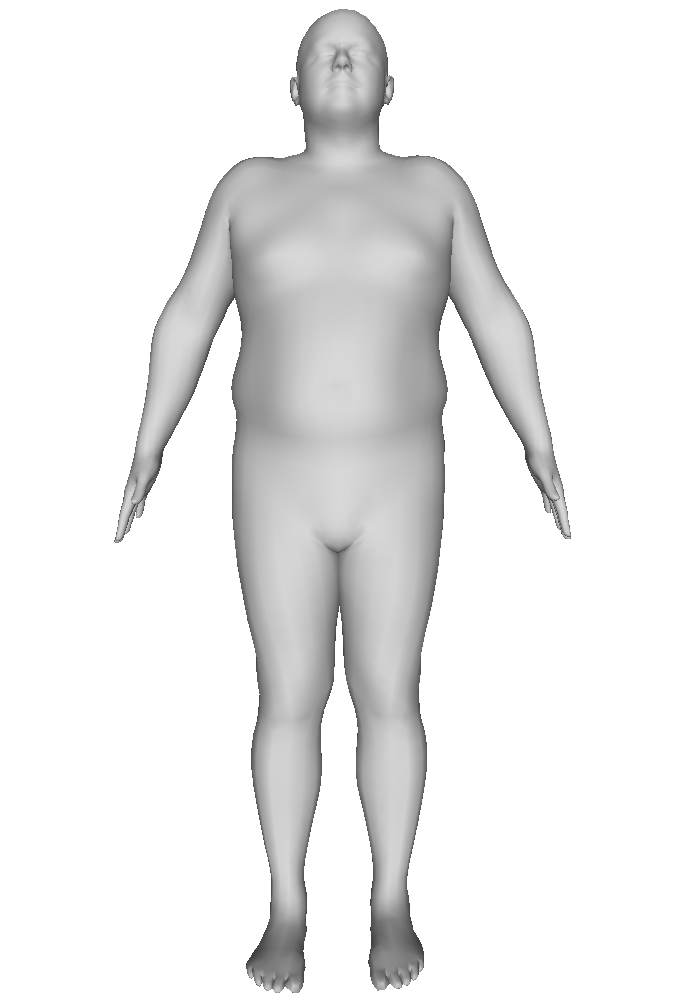
\includegraphics[width=75pt]{files/patient_8/2_cropped}
      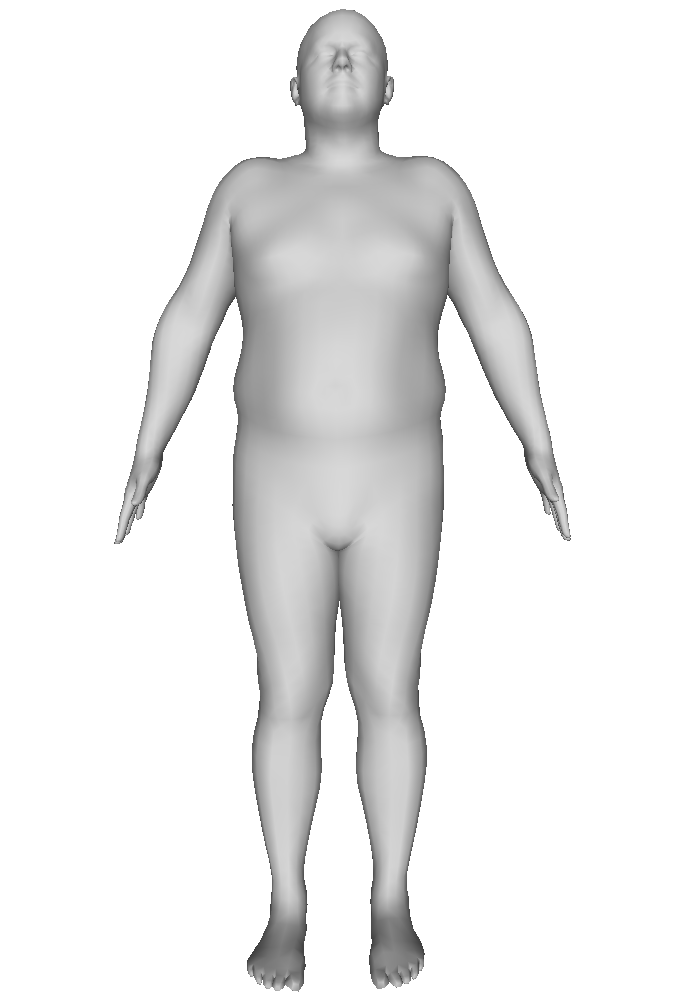
\includegraphics[width=75pt]{files/patient_8/3_cropped}
      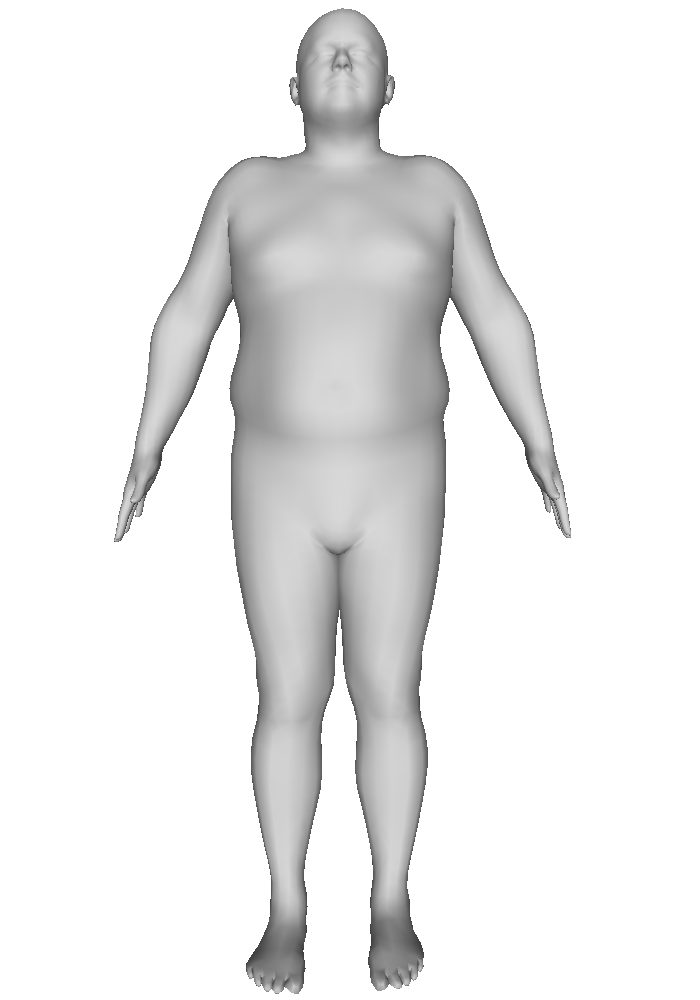
\includegraphics[width=75pt]{files/patient_8/4_cropped}
      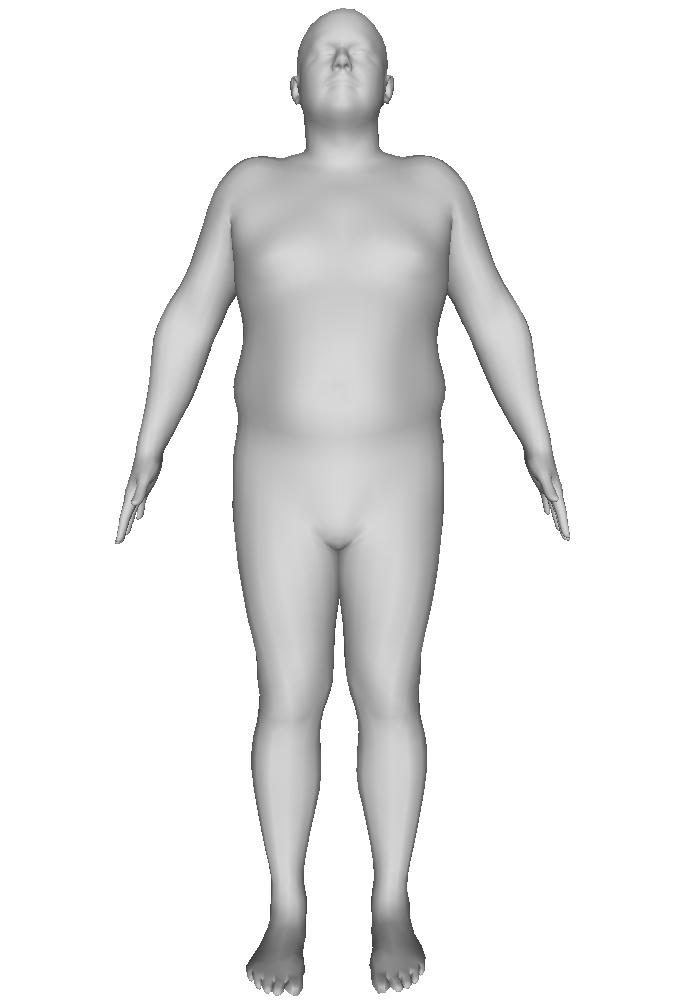
\includegraphics[width=75pt]{files/patient_8/5_cropped}
      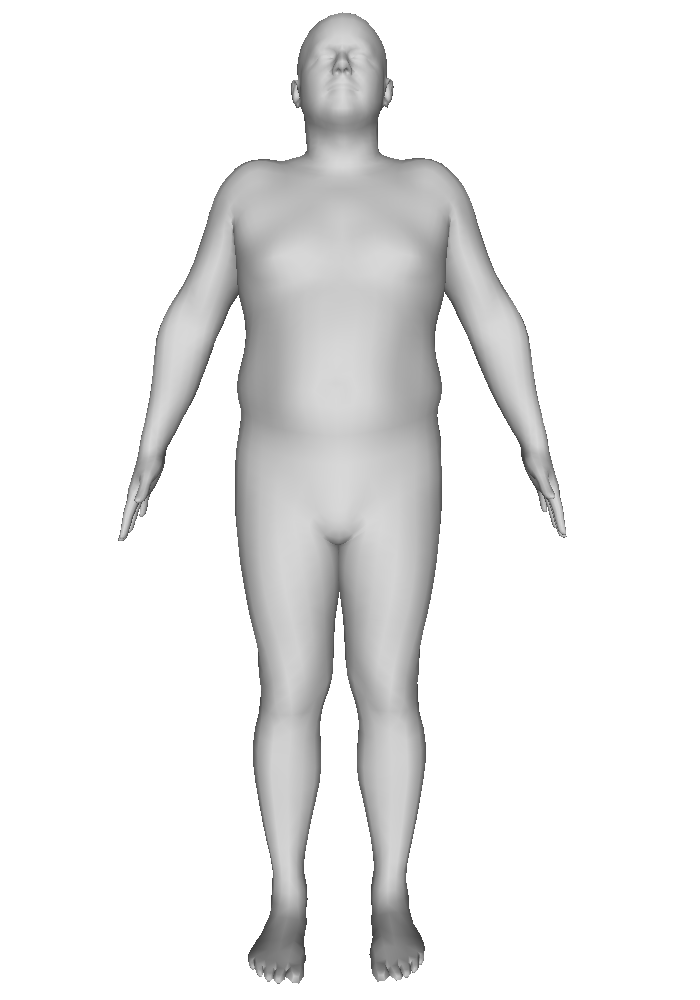
\includegraphics[width=75pt]{files/patient_8/6_cropped}
      \caption{3D model reconstruction of a patient's body at different stages of a weight loss
            treatment. There is around a month between each scan, and a total
            weight loss of 3.8 kg.}
\end{figure}

Subsequently, we wondered if it would be feasible to utilize the datasets
acquired in this prior study to formulate a predictive model. This model would
project anticipated changes in a person's body undergoing weight loss treatment
before the treatment concludes, further bolstering adherence to the treatment
regimen. The present work explores the development of such a model. This
includes analyzing data from the earlier study, reviewing existing techniques
in human body model representation, encoding patient data using the chosen
representation, devising a neural network architecture for predicting patient
body changes, and finally, training and evaluating the model.

\section{3D human body model applications}

There are many areas that can make use of these models. Some of the most
significant applications include:

\begin{itemize}
      \item Medicine: Human body models are valuable in the study of
            anatomy~\cite{https://doi.org/10.1002/ase.1718} and for patient monitoring.
      \item Film industry: Human body models can be used to capture motion data and render
            high-quality CGI humans.
      \item Video game industry: Human body models can be used to create realistic
            animations and interactions between characters\cite{Starke2021}.
      \item Extended reality: Human body models can be used to capture user input in
            virtual reality as well as rendering realistic characters.
      \item Clothing: These models can be used for fitting virtual
            clothes\cite{apeagyei2010application} and creating realistic images of clothing
            products.
\end{itemize}
%%%%%%%%%%%%%%%%%%%%%%%%%%%%%%%%%%%%%%%%%%%%%%%%%%%%%%%%%%%%%%%%%%%%%%%%
% Plantilla TFG/TFM
% Escuela Politécnica Superior de la Universidad de Alicante
% Realizado por: Jose Manuel Requena Plens
% Contacto: info@jmrplens.com / Telegram:@jmrplens
%%%%%%%%%%%%%%%%%%%%%%%%%%%%%%%%%%%%%%%%%%%%%%%%%%%%%%%%%%%%%%%%%%%%%%%%

\chapter{State of the Art}\label{stateoftheart}

The first step in predicting how a human body will evolve over time involves
representing it in a format comprehensible to a computer. Numerous methods
exist for this, each offering distinct advantages and drawbacks. This chapter
will delve into several of the most prevalent ways to represent a human body in
3D space. Our research on this subject culminated in the submission of a paper
to the IWANN 2023 conference.

\section{3D human body representation}

A straightforward approach to categorize human body representations is to
classify based on the required input type and the generated output.

\subsection{Input}

Regarding input, representations fall into two main categories. categories:

\begin{itemize}
    \item 2D input: These representations utilize 2D images or videos as input. Some models may also process images from varying angles. The flexibility of these models is beneficial as they do not necessitate specific hardware to capture the input data.
    \item 3D input: Typically, these models require 3D point clouds as input data.
    \item Parametric models: These models demand a set of parameters describing the body.
          Some models categorize these parameters into body shape and body pose. This
          form of representation is highly intriguing for machine learning applications
          due to the significant reduction in input data dimensionality. This factor
          permits the training of a neural network with fewer samples. However, it
          necessitates a model capable of generating parameters from the input data.
\end{itemize}

\subsection{Output}

\subsubsection{Human specific}

Certain models generate 3D meshes of the human body compatible with blend
skinning, enabling animation with a skeleton. This feature proves invaluable
for applications like video games or cinematic productions.

\subsubsection{General}

These models can generate 3D representations of any object, not just humans.

\begin{itemize}
    \item 3D meshes: These models create a 3D mesh of the object.
    \item 3D voxel: These models produce a 3D voxel grid of the object. However, this approach is not widespread as it is generally not beneficial for most applications.
    \item \gls{nerf}: This novel 3D representation directly renders the object from a specific viewpoint. While this allows for the generation of highly realistic images, it proves less beneficial for applications requiring a true 3D representation of the object.
\end{itemize}
%%%%%%%%%%%%%%%%%%%%%%%%%%%%%%%%%%%%%%%%%%%%%%%%%%%%%%%%%%%%%%%%%%%%%%%%
% Plantilla TFG/TFM
% Escuela Politécnica Superior de la Universidad de Alicante
% Realizado por: Jose Manuel Requena Plens
% Contacto: info@jmrplens.com / Telegram:@jmrplens
%%%%%%%%%%%%%%%%%%%%%%%%%%%%%%%%%%%%%%%%%%%%%%%%%%%%%%%%%%%%%%%%%%%%%%%%

\chapter{Objectives}\label{objectives}

Explore techniques to represent a human body in 3D space and compare them.

Design and implement a neural network that can understand human bodies and
train it to predict shape changes in time.

Use the neural network to generate 3D meshes of the predicted models.

\todo[]{
    Este es un punto muy importante para el lector.
    Sobretodo para el tribunal.
    Tienen que quedar claros los sub-objetos que nos hemos marcado
    y el objetivo principal del TFG.\@
    Puedes utilizar mi TFG o TFM como plantilla
}
%%%%%%%%%%%%%%%%%%%%%%%%%%%%%%%%%%%%%%%%%%%%%%%%%%%%%%%%%%%%%%%%%%%%%%%%
% Plantilla TFG/TFM
% Escuela Politécnica Superior de la Universidad de Alicante
% Realizado por: Jose Manuel Requena Plens
% Contacto: info@jmrplens.com / Telegram:@jmrplens
%%%%%%%%%%%%%%%%%%%%%%%%%%%%%%%%%%%%%%%%%%%%%%%%%%%%%%%%%%%%%%%%%%%%%%%%

\chapter{Methodology}\label{methodology}

\section{Data}

Our data comprises approximately 400 sessions collected from 80 patients. These
sessions were recorded at various time points and are not uniformly spaced.
Each session's data includes a 3D scan of the patient, along with several
measurements such as weight, height, body fat percentage, etc.

\todo[]{Puedes añadir la tabla que aparece en el paper A Non-Invasive Approach for Total Cholesterol Level Prediction Using Machine Learning}

\todo[]{${https://rua.ua.es/dspace/bitstream/10045/124160/6/Garcia-dUrso_etal_2022_IEEEAccess.pdf}$}

However, the data requires cleaning before usage. Some sessions lack certain
measurements, and there are numerous outliers within the data. After cleaning,
we utilized about 200 sessions.

\todo[]{Puedes añadir un sub-punto hablando del preprocesado de los datos}

\section{Body representation}

In order to represent the body shape we opted to use \gls{smpl}. \gls{smpl}
encodes the body shape and pose using a low-dimensional linear space. The body
shape is encoded using 10 shape parameters ($\beta$), and the pose is encoded
using 72 pose parameters ($\theta$). As our interest lies in body shape, we
employed only the shape parameters.

\def\betaVar{3}
\def\imgWidth{0.3\textwidth}
\def\betaWidth{\textwidth}

\begin{figure}[ht!]
    \centering
    \begin{minipage}[b]{\textwidth}
        \centering
        \includegraphics[width=\imgWidth]{files/visualize_betas/beta_0_-\betaVar_m}
        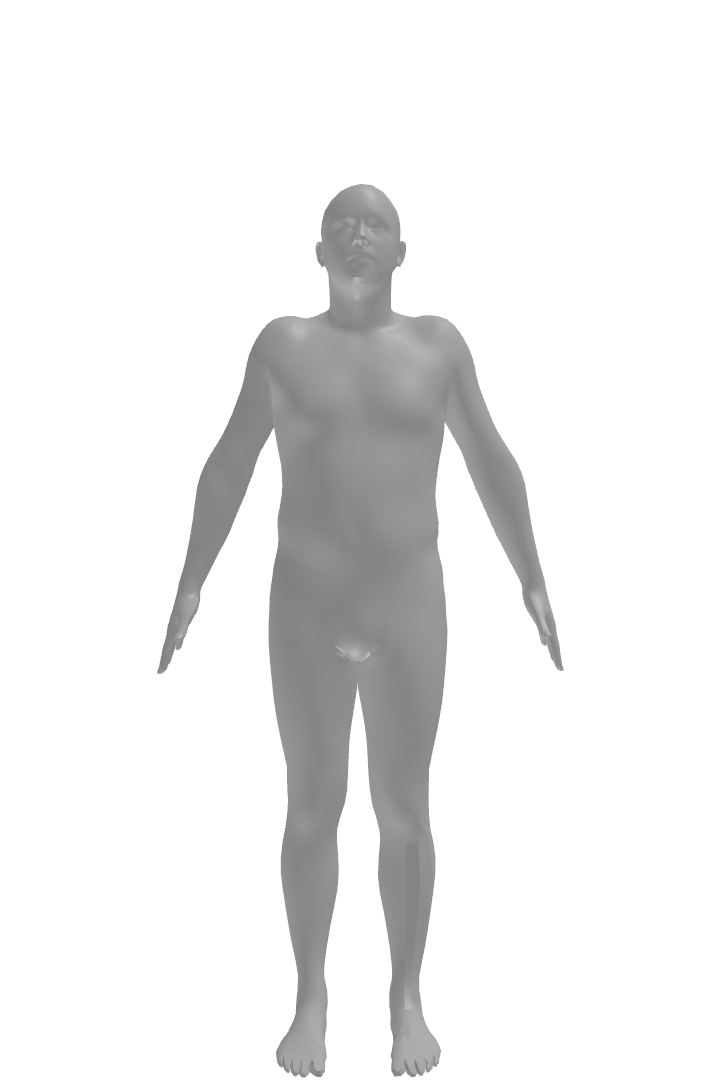
\includegraphics[width=\imgWidth]{files/visualize_betas/baseline_m}
        \includegraphics[width=\imgWidth]{files/visualize_betas/beta_0_\betaVar_m}
        \linebreak
        \includegraphics[width=\imgWidth]{files/visualize_betas/beta_0_-\betaVar_f}
        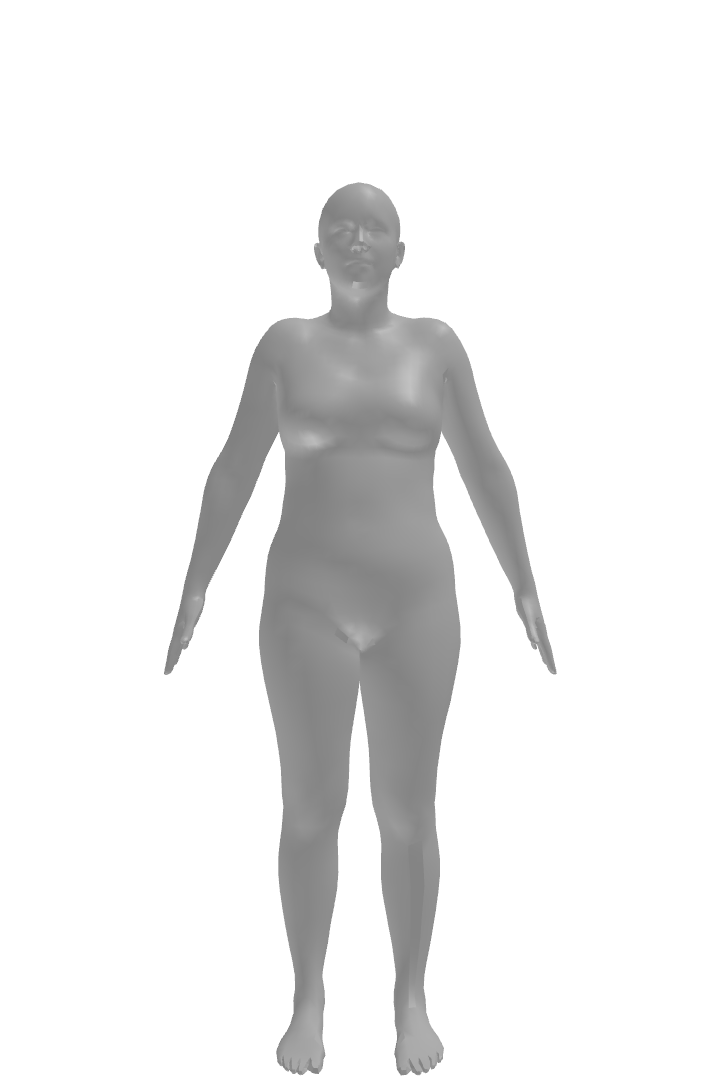
\includegraphics[width=\imgWidth]{files/visualize_betas/baseline_f}
        \includegraphics[width=\imgWidth]{files/visualize_betas/beta_0_\betaVar_f}
        \caption[Effect of varying $\beta_1$ in SMPL.]{$\beta_1 = [-\betaVar, 0, +\betaVar]$.}
        \label{fig:beta-1-vis}
    \end{minipage}
\end{figure}

\begin{figure}[ht!]
    \centering

    \begin{minipage}[b]{\textwidth}
        \centering
        \includegraphics[width=\imgWidth]{files/visualize_betas/beta_1_-\betaVar_m}
        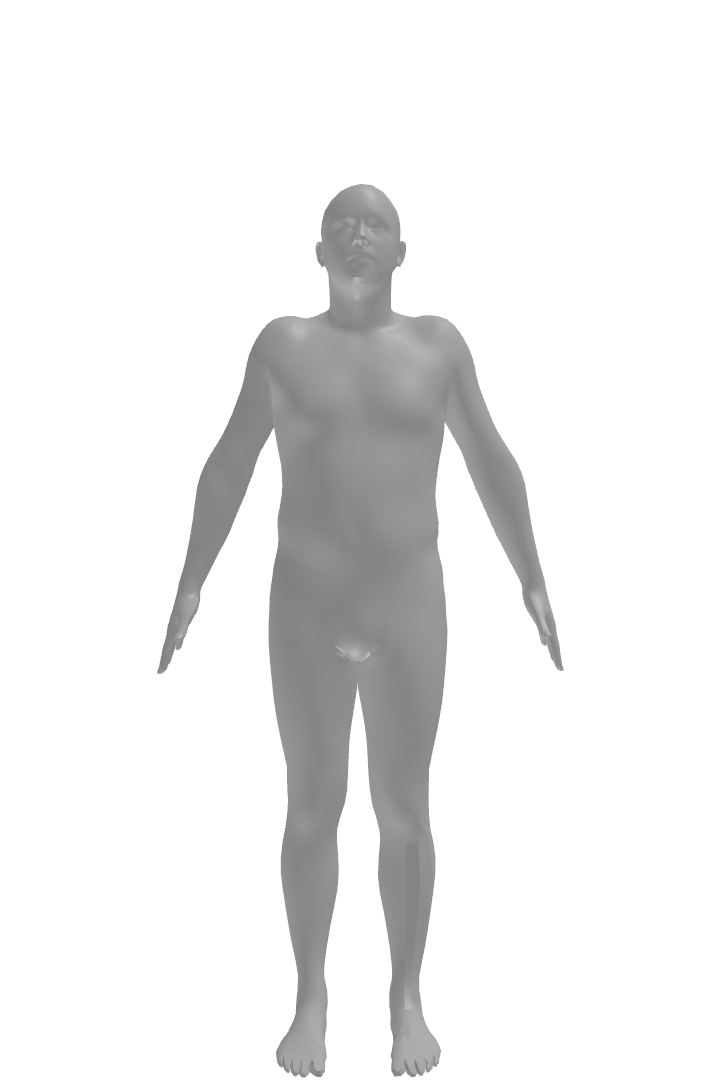
\includegraphics[width=\imgWidth]{files/visualize_betas/baseline_m}
        \includegraphics[width=\imgWidth]{files/visualize_betas/beta_1_\betaVar_m}
        \linebreak
        \includegraphics[width=\imgWidth]{files/visualize_betas/beta_1_-\betaVar_f}
        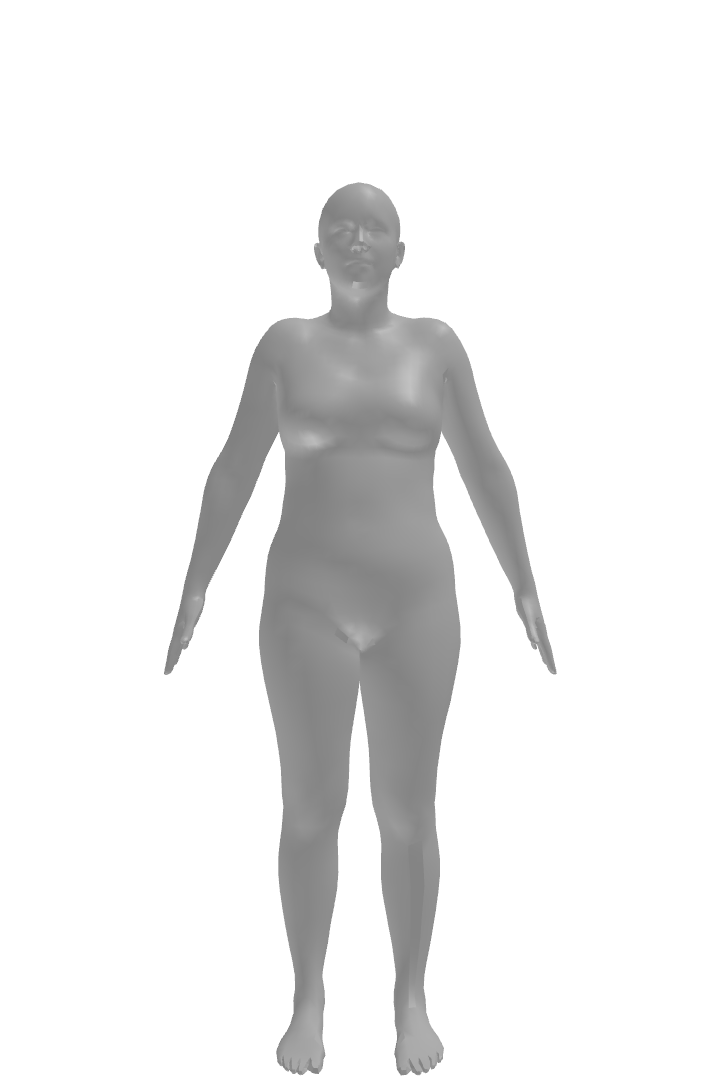
\includegraphics[width=\imgWidth]{files/visualize_betas/baseline_f}
        \includegraphics[width=\imgWidth]{files/visualize_betas/beta_1_\betaVar_f}
        \caption[Effect of varying $\beta_2$ in SMPL.]{$\beta_2 = [-\betaVar, 0, +\betaVar]$.}
    \end{minipage}
\end{figure}

\begin{figure}[ht!]
    \centering

    \begin{minipage}[b]{\textwidth}
        \centering
        \includegraphics[width=\imgWidth]{files/visualize_betas/beta_2_-\betaVar_m}
        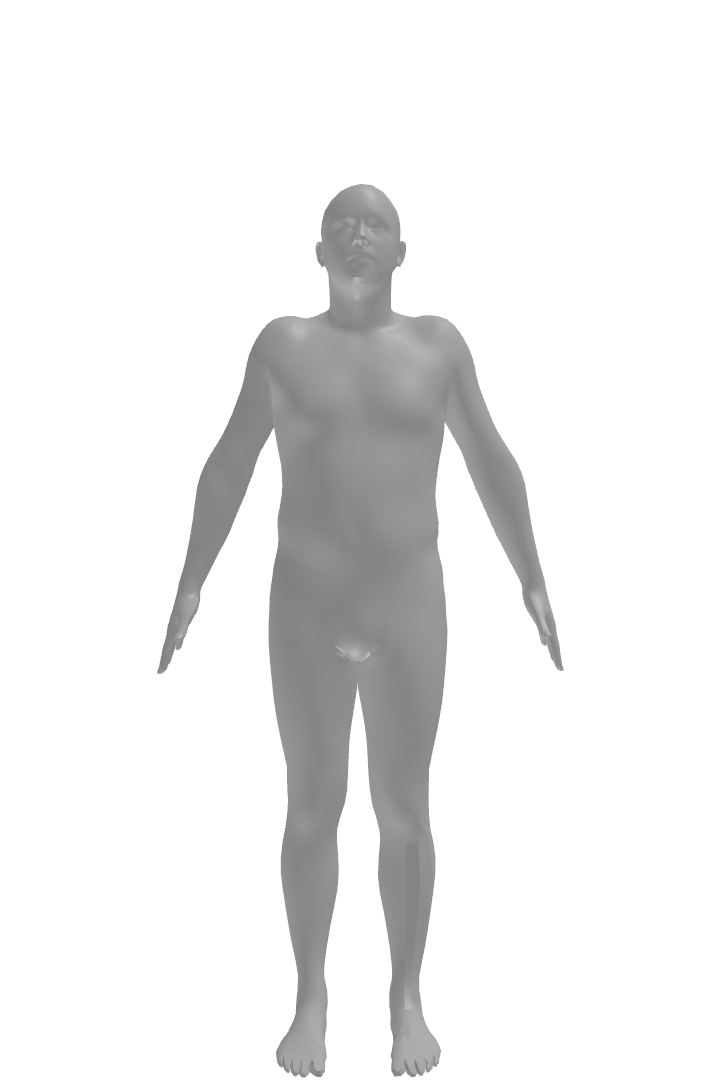
\includegraphics[width=\imgWidth]{files/visualize_betas/baseline_m}
        \includegraphics[width=\imgWidth]{files/visualize_betas/beta_2_\betaVar_m}
        \linebreak
        \includegraphics[width=\imgWidth]{files/visualize_betas/beta_2_-\betaVar_f}
        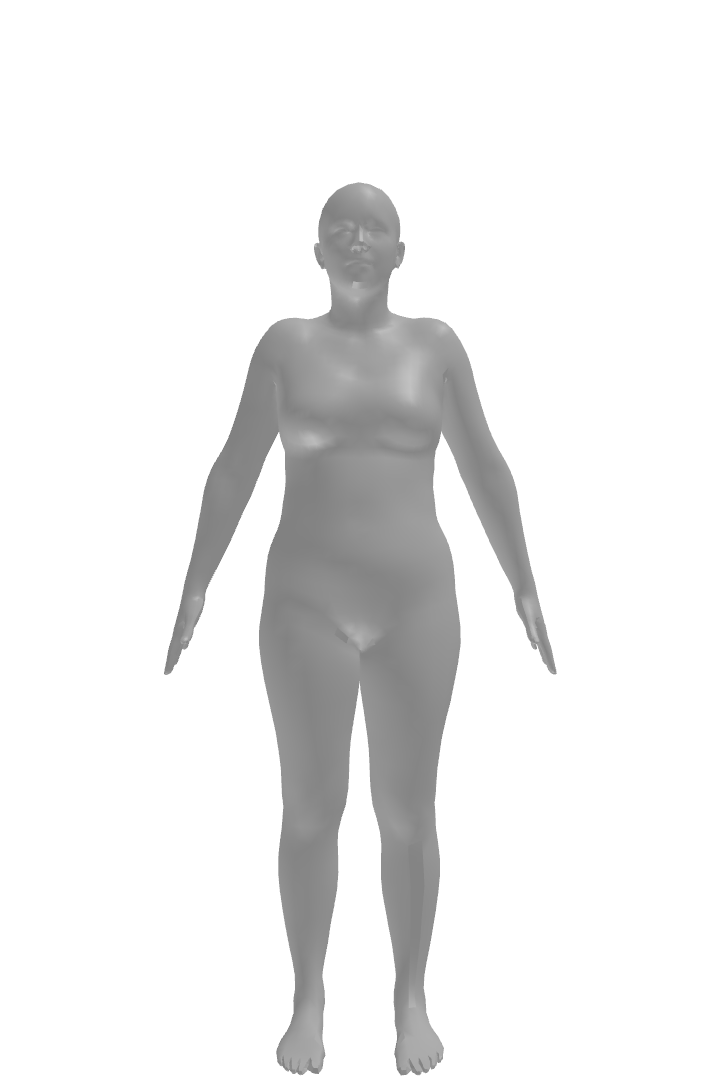
\includegraphics[width=\imgWidth]{files/visualize_betas/baseline_f}
        \includegraphics[width=\imgWidth]{files/visualize_betas/beta_2_\betaVar_f}
        \caption[Effect of varying $\beta_3$ in SMPL.]{$\beta_3 = [-\betaVar, 0, +\betaVar]$.}
    \end{minipage}
\end{figure}

\begin{figure}[ht!]
    \centering

    \begin{minipage}[b]{\textwidth}
        \centering
        \includegraphics[width=\imgWidth]{files/visualize_betas/beta_3_-\betaVar_m}
        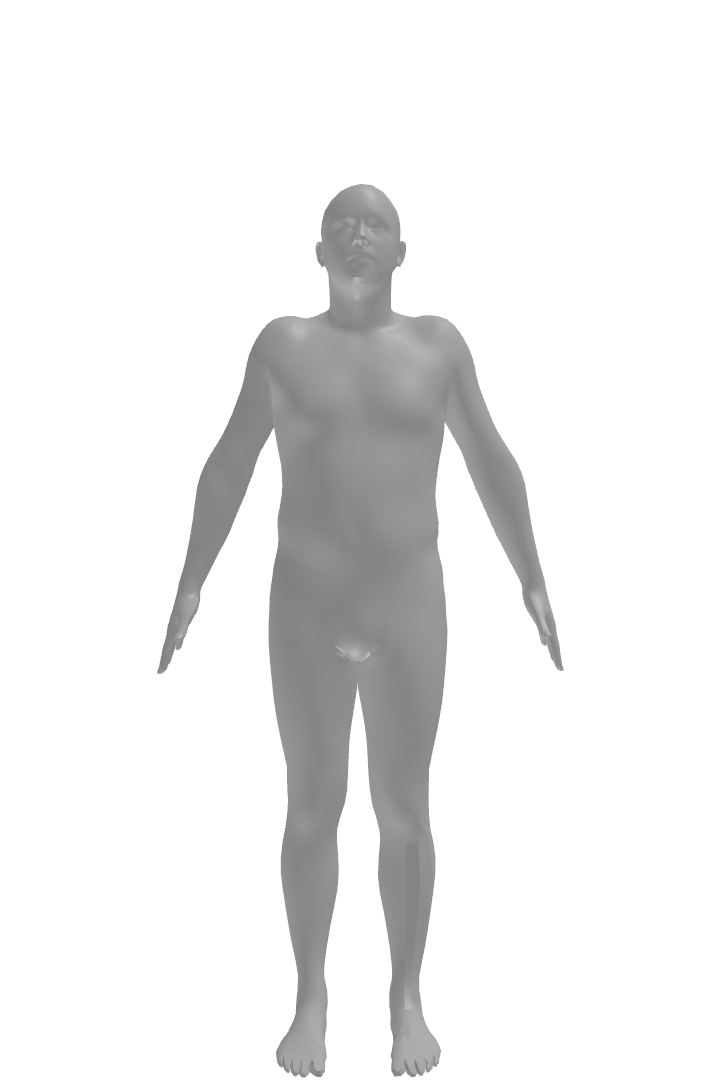
\includegraphics[width=\imgWidth]{files/visualize_betas/baseline_m}
        \includegraphics[width=\imgWidth]{files/visualize_betas/beta_3_\betaVar_m}
        \linebreak
        \includegraphics[width=\imgWidth]{files/visualize_betas/beta_3_-\betaVar_f}
        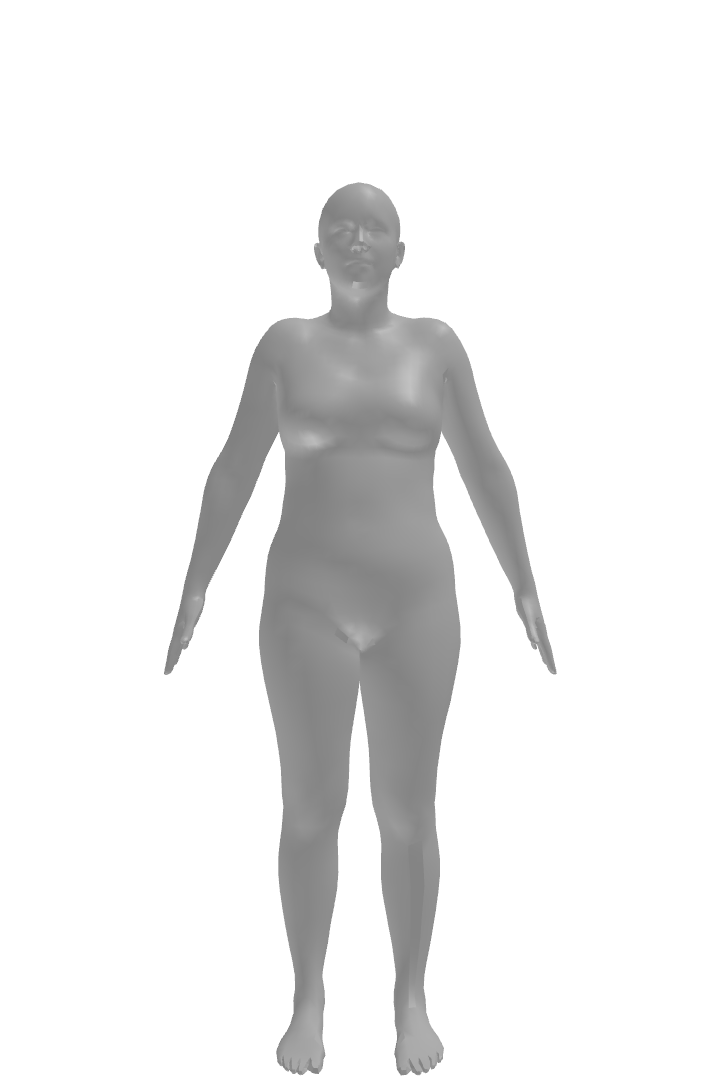
\includegraphics[width=\imgWidth]{files/visualize_betas/baseline_f}
        \includegraphics[width=\imgWidth]{files/visualize_betas/beta_3_\betaVar_f}
        \caption[Effect of varying $\beta_4$ in SMPL.]{$\beta_4 = [-\betaVar, 0, +\betaVar]$.}
    \end{minipage}
\end{figure}

\begin{figure}[ht!]
    \centering

    \begin{minipage}[b]{\textwidth}
        \centering
        \includegraphics[width=\imgWidth]{files/visualize_betas/beta_4_-\betaVar_m}
        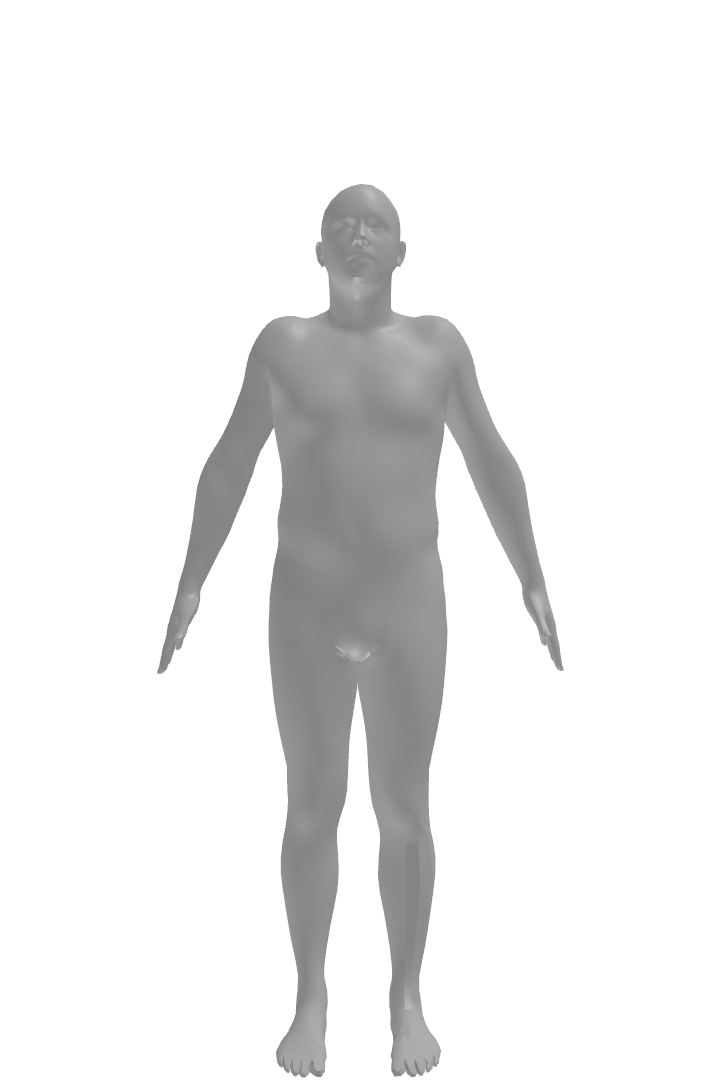
\includegraphics[width=\imgWidth]{files/visualize_betas/baseline_m}
        \includegraphics[width=\imgWidth]{files/visualize_betas/beta_4_\betaVar_m}
        \linebreak
        \includegraphics[width=\imgWidth]{files/visualize_betas/beta_4_-\betaVar_f}
        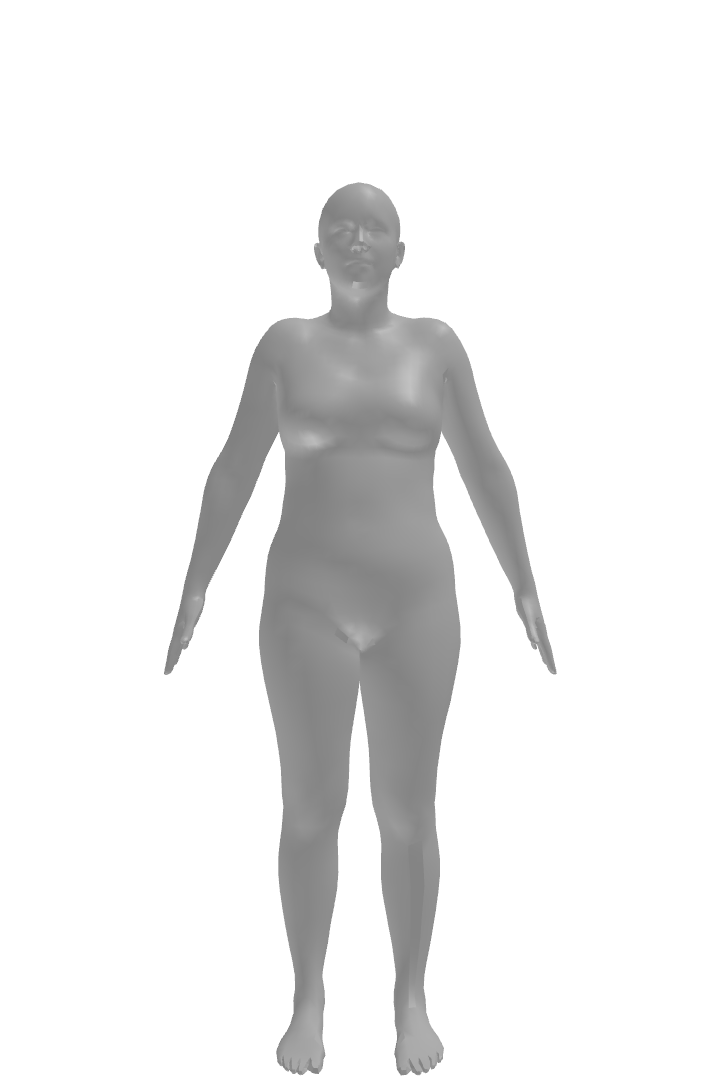
\includegraphics[width=\imgWidth]{files/visualize_betas/baseline_f}
        \includegraphics[width=\imgWidth]{files/visualize_betas/beta_4_\betaVar_f}
        \caption[Effect of varying $\beta_5$ in SMPL.]{$\beta_5 = [-\betaVar, 0, +\betaVar]$.}
    \end{minipage}
\end{figure}

\begin{figure}[ht!]
    \centering

    \begin{minipage}[b]{\textwidth}
        \centering
        \includegraphics[width=\imgWidth]{files/visualize_betas/beta_5_-\betaVar_m}
        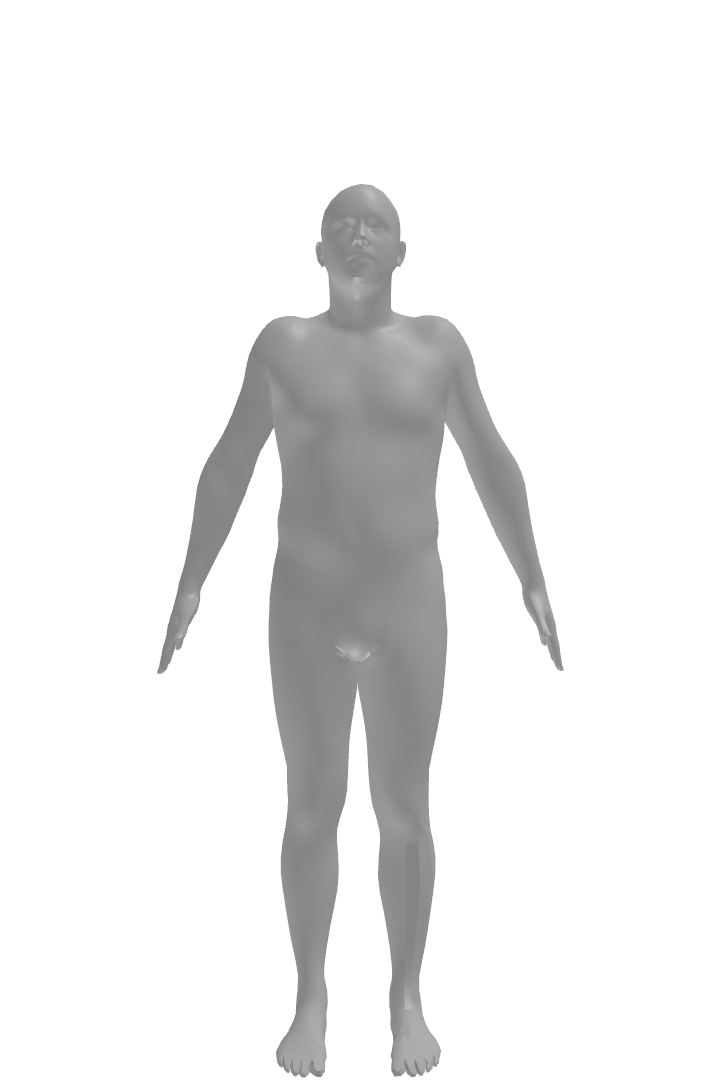
\includegraphics[width=\imgWidth]{files/visualize_betas/baseline_m}
        \includegraphics[width=\imgWidth]{files/visualize_betas/beta_5_\betaVar_m}
        \linebreak
        \includegraphics[width=\imgWidth]{files/visualize_betas/beta_5_-\betaVar_f}
        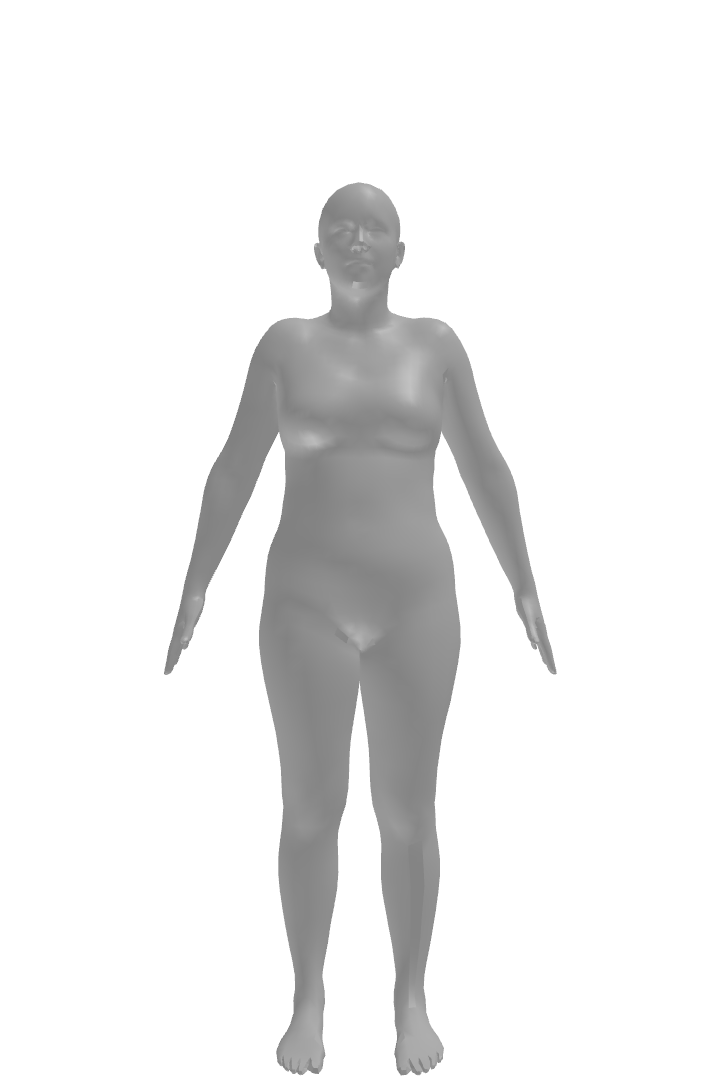
\includegraphics[width=\imgWidth]{files/visualize_betas/baseline_f}
        \includegraphics[width=\imgWidth]{files/visualize_betas/beta_5_\betaVar_f}
        \caption[Effect of varying $\beta_6$ in SMPL.]{$\beta_6 = [-\betaVar, 0, +\betaVar]$.}
    \end{minipage}
\end{figure}

\begin{figure}[ht!]
    \centering

    \begin{minipage}[b]{\textwidth}
        \centering
        \includegraphics[width=\imgWidth]{files/visualize_betas/beta_6_-\betaVar_m}
        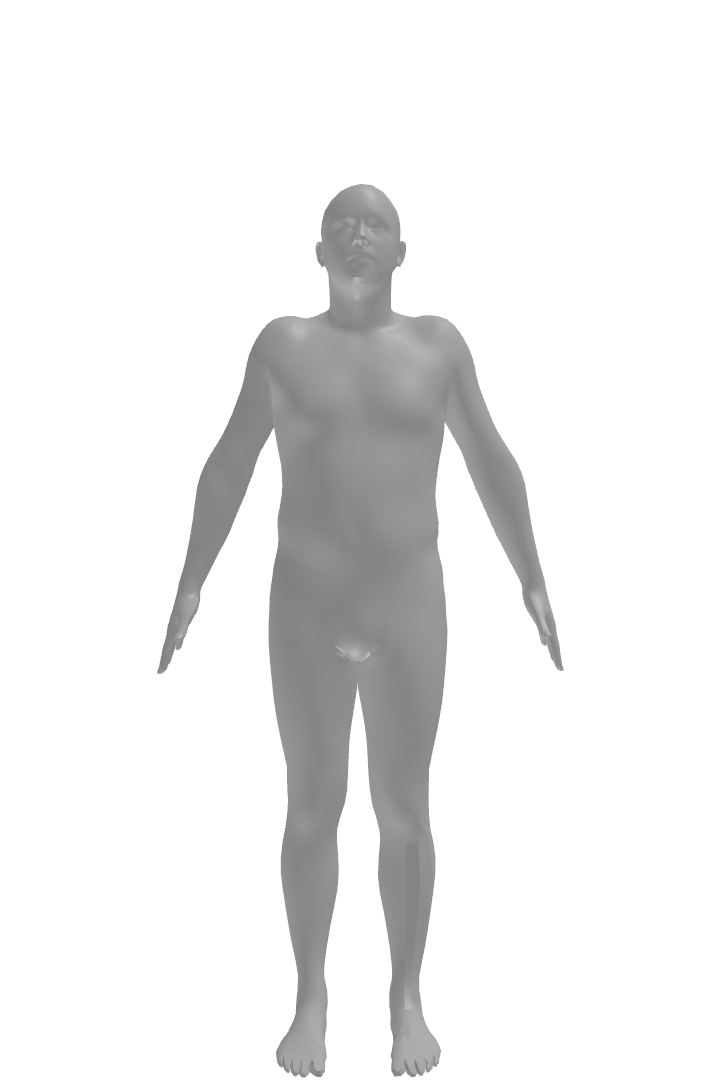
\includegraphics[width=\imgWidth]{files/visualize_betas/baseline_m}
        \includegraphics[width=\imgWidth]{files/visualize_betas/beta_6_\betaVar_m}
        \linebreak
        \includegraphics[width=\imgWidth]{files/visualize_betas/beta_6_-\betaVar_f}
        \includegraphics[width=\imgWidth]{files/visualize_betas/baseline_f}
        \includegraphics[width=\imgWidth]{files/visualize_betas/beta_6_\betaVar_f}
        \caption[Effect of varying $\beta_7$ in SMPL.]{$\beta_7 = [-\betaVar, 0, +\betaVar]$.}
    \end{minipage}
\end{figure}

\begin{figure}[ht!]
    \centering

    \begin{minipage}[b]{\textwidth}
        \centering
        \includegraphics[width=\imgWidth]{files/visualize_betas/beta_7_-\betaVar_m}
        \includegraphics[width=\imgWidth]{files/visualize_betas/baseline_m}
        \includegraphics[width=\imgWidth]{files/visualize_betas/beta_7_\betaVar_m}
        \linebreak
        \includegraphics[width=\imgWidth]{files/visualize_betas/beta_7_-\betaVar_f}
        \includegraphics[width=\imgWidth]{files/visualize_betas/baseline_f}
        \includegraphics[width=\imgWidth]{files/visualize_betas/beta_7_\betaVar_f}
        \caption[Effect of varying $\beta_8$ in SMPL.]{$\beta_8 = [-\betaVar, 0, +\betaVar]$.}
    \end{minipage}
\end{figure}

\begin{figure}[ht!]
    \centering

    \begin{minipage}[b]{\textwidth}
        \centering
        \includegraphics[width=\imgWidth]{files/visualize_betas/beta_8_-\betaVar_m}
        \includegraphics[width=\imgWidth]{files/visualize_betas/baseline_m}
        \includegraphics[width=\imgWidth]{files/visualize_betas/beta_8_\betaVar_m}
        \linebreak
        \includegraphics[width=\imgWidth]{files/visualize_betas/beta_8_-\betaVar_f}
        \includegraphics[width=\imgWidth]{files/visualize_betas/baseline_f}
        \includegraphics[width=\imgWidth]{files/visualize_betas/beta_8_\betaVar_f}
        \caption[Effect of varying $\beta_9$ in SMPL.]{$\beta_9 = [-\betaVar, 0, +\betaVar]$.}
    \end{minipage}
\end{figure}

\begin{figure}[ht!]
    \centering

    \begin{minipage}[b]{\textwidth}
        \centering
        \includegraphics[width=\imgWidth]{files/visualize_betas/beta_9_-\betaVar_m}
        \includegraphics[width=\imgWidth]{files/visualize_betas/baseline_m}
        \includegraphics[width=\imgWidth]{files/visualize_betas/beta_9_\betaVar_m}
        \linebreak
        \includegraphics[width=\imgWidth]{files/visualize_betas/beta_9_-\betaVar_f}
        \includegraphics[width=\imgWidth]{files/visualize_betas/baseline_f}
        \includegraphics[width=\imgWidth]{files/visualize_betas/beta_9_\betaVar_f}
        \caption[Effect of varying $\beta_{10}$ in SMPL.]{$\beta_{10} = [-\betaVar, 0, +\betaVar]$.}
        \label{fig:beta-10-vis}
    \end{minipage}
\end{figure}


Figure~\ref{fig:beta-vis} shows the effect of varying the shape parameters. We
have used a scale of 3 to better show their effect, but in practice the values
are much smaller. $\beta_0$ controls the overall height of the body, while
$\beta_1$ has a large correlation with the body mass index.

\begin{table}[h]
    \centering
    \begin{tabular}{ |c|c|c|c|c|c|c|c|c|c|c| }
        \hline
             & $\beta_1$ & $\beta_2$ & $\beta_3$ & $\beta_4$ & $\beta_5$ & $\beta_6$ & $\beta_7$ & $\beta_8$ & $\beta_9$ & $\beta_{10}$ \\
        \hline
        mean & 0.88      & -0.73     & 0.34      & 0.01      & 0.06      & 0.06      & 0.11      & 0.02      & 0.01      & 0.11         \\
        \hline
        std  & 0.97      & 0.78      & 0.26      & 0.21      & 0.12      & 0.13      & 0.08      & 0.03      & 0.03      & 0.08         \\
        \hline
        min  & -1.42     & -2.57     & -0.64     & -0.65     & -0.23     & -0.25     & -0.14     & -0.07     & -0.08     & -0.17        \\
        \hline
        25\% & 0.12      & -1.26     & 0.15      & -0.14     & -0.01     & -0.02     & 0.04      & 0.00      & -0.01     & 0.06         \\
        \hline
        50\% & 0.94      & -0.69     & 0.36      & 0.03      & 0.04      & 0.02      & 0.11      & 0.02      & 0.01      & 0.11         \\
        \hline
        75\% & 1.66      & -0.20     & 0.52      & 0.17      & 0.14      & 0.14      & 0.16      & 0.04      & 0.04      & 0.17         \\
        \hline
        max  & 2.90      & 2.96      & 0.97      & 0.45      & 0.39      & 0.47      & 0.36      & 0.13      & 0.16      & 0.30         \\
        \hline
    \end{tabular}
    \caption{Statistics of the shape parameters}
\end{table}

\section{Neural network architecture}

Given the nature of the data, we decided to use a neural network to predict the
changes in the body shape. Since the data is temporal, we need to use a neural
network architecture that can handle temporal data.

There are different neural network architectures that work well with temporal
data. Recurrent neural networks are a type of neural networks that feed the
output of the previous step as input to the next step. This allows them to
remember information from previous steps, which is useful for time series.
However, they can `forget' information from the beginning of the sequence,
which is a problem known as vanishing gradients. There are some variations of
recurrent neural networks that try to solve this problem, such as \gls{lstm}
and \gls{gru}.

Transformer networks are a relatively new type of neural network that has been
used with great success in natural language processing. They are based on
attention mechanisms, which allow them to focus on specific parts of the input
sequence. This makes them very useful for time series, since they can focus on
the most relevant parts of the sequence. The big disadvantage of transformer
networks for this application is that they require large amounts of training
data\todo[]{citation needed}, which is not available in this case.

We ended up using an neural network architecture that uses an \gls{lstm}.

\section{Training}

\subsection{Variability in the dates of the sessions}

The dataset's sessions are not uniformly spaced in time, varying from a few
days to several months apart. To mitigate this issue, we:

Calculated a variable representing the number of days until the next session.

Modified the neural network to predict the daily change in variables, instead
of predicting the variables for the following session.

We implemented a residual connection to the neural network, enabling it to
predict the change in variables from one session to the next. Then, we
multiplied this change by the number of days until the next session and added
it to the previous session to calculate the predicted values for the next
session. This approach assumes a linear change between sessions—an
approximation suited to our purpose. We augmented the data by randomly removing
intermediate sessions and recalculating the number of days until the next
session.

\section{Evaluation}

\section{Results}	
%%%%%%%%%%%%%%%%%%%%%%%%%%%%%%%%%%%%%%%%%%%%%%%%%%%%%%%%%%%%%%%%%%%%%%%%
% Plantilla TFG/TFM
% Escuela Politécnica Superior de la Universidad de Alicante
% Realizado por: Jose Manuel Requena Plens
% Contacto: info@jmrplens.com / Telegram:@jmrplens
%%%%%%%%%%%%%%%%%%%%%%%%%%%%%%%%%%%%%%%%%%%%%%%%%%%%%%%%%%%%%%%%%%%%%%%%

\chapter{Development}\label{development}
\section{Data}

We developed a data cleaning pipeline using the pandas library. This pipeline
fixes some errors in the data, removes outliers and sessions with missing
measurements.

\section{Body representation}

We extracted \gls{smpl} parameters --- shape ($\beta$) and pose ($\theta$) ---
from the 3D scans using a custom minimization algorithm.

\section{Neural network architecture}

We used the PyTorch library to implement our custom neural network
architecture.

\begin{figure}
    \centering
    \includegraphics[width=6cm]{files/nn_diagram}
    \caption{Diagram of the neural network architecture}
\end{figure}

This architecture can handle temporal data of varying lengths.

\section{Training}

The neural network inputs a tensor of shape (batch size, max sequence length,
number of features), a tensor of shape (batch size, 1) containing the length of
the current sequence, and a scalar representing the number of days until the
next session. It returns a tensor of shape (batch size, max sequence length,
number of features) containing the predicted values for the next session.

\begin{itemize}
    \item The neural network takes as input:
          \begin{itemize}
              \item A tensor of shape (batch size, max sequence length, number of features).
              \item A tensor of shape (batch size, 1) containing the length of the current
                    sequence.
              \item A scalar representing the number of days until the next session.
          \end{itemize}
    \item The neural network returns:
          \begin{itemize}
              \item A tensor of shape (batch size, max sequence length, number of features) that
                    contains the predicted values for the next session.
          \end{itemize}
\end{itemize}

For features, we concatenate the \gls{smpl} parameters shape ($\beta$) with the
patient's height, weight, and age. We also experimented with using body fat
percentage and muscle mass percentage, but the results were comparable. We used
the AdamW optimizer with a variable learning rate and weight decay, and MSE
loss.

\section{Evaluation}

The mean absolute error (MAE) of the predicted betas served as our evaluation
metric.

\section{Results}

\begin{figure}[h]
    \centering
    \includegraphics[width=\textwidth]{files/predicted_betas}
    \caption{Change of the shape parameters for a given patient and the neural
        network prediction after 30 days}
\end{figure}
%%%%%%%%%%%%%%%%%%%%%%%%%%%%%%%%%%%%%%%%%%%%%%%%%%%%%%%%%%%%%%%%%%%%%%%%
% Plantilla TFG/TFM
% Escuela Politécnica Superior de la Universidad de Alicante
% Realizado por: Jose Manuel Requena Plens
% Contacto: info@jmrplens.com / Telegram:@jmrplens
%%%%%%%%%%%%%%%%%%%%%%%%%%%%%%%%%%%%%%%%%%%%%%%%%%%%%%%%%%%%%%%%%%%%%%%%

\chapter{Results}\label{results}
%%%%%%%%%%%%%%%%%%%%%%%%%%%%%%%%%%%%%%%%%%%%%%%%%%%%%%%%%%%%%%%%%%%%%%%%
% Plantilla TFG/TFM
% Escuela Politécnica Superior de la Universidad de Alicante
% Realizado por: Jose Manuel Requena Plens
% Contacto: info@jmrplens.com / Telegram:@jmrplens
%%%%%%%%%%%%%%%%%%%%%%%%%%%%%%%%%%%%%%%%%%%%%%%%%%%%%%%%%%%%%%%%%%%%%%%%

\chapter{Conclusion}\label{conclusion}

This work has paved the way for an innovative approach to predicting changes in
body shape during weight loss treatment, using machine learning models and the
data gathered from the previous study. Our prediction model based on \gls{smpl}
and a \gls{lstm}-based neural network successfully demonstrated its ability to
approximate the expected changes in body shape before the conclusion of the
weight loss treatment, which could potentially lead to improved adherence to
treatment plans.

However, our study was not without limitations. The model's performance was
constrained by the quantity and quality of data available. Our dataset
consisted of approximately 200 sessions from 80 patients, which, while
substantial, might not fully capture the wide range of variability in human
body shapes and weight loss patterns. Moreover, outliers and missing data,
which had to be cleaned from our dataset, posed additional challenges.

In future work, several improvements and expansions can be explored:

\begin{itemize}
    \item \textbf{Data collection}: Patients could submit images instead of requiring 3D scans. This approach would allow for increased data collection, while also reducing friction for the patient. We can also consider developing a method to generate 3D models from these images.
    \item \textbf{Neural network architecture}: While we opted for a \gls{lstm}
          architecture due to the nature of our data, other neural network architectures,
          such as Transformers, could be explored for potential improvements in
          prediction performance.
    \item \textbf{Parametric models}: Other parametric models like STAR could
          be considered as alternatives or complements to the \gls{smpl}
          model we used. They might offer different advantages or better fit
          the data depending on the specific conditions and requirements.

    \item \textbf{Rendering output}: An exploration of smplpix for 2D
          rendering output might provide an alternative approach for generating
          visualization of predicted body changes.
\end{itemize}

%%%%
% CONTENIDO. BIBLIOGRAFÍA.
%%%%
\nocite{*} %incluye TODOS los documentos de la base de datos bibliográfica sean o no citados en el texto
\bibliography{bibliography/bibliography} % Archivo que contiene la bibliografía
\bibliographystyle{apacite}

%%%%
% CONTENIDO. LISTA DE ACRÓNIMOS. Comenta las líneas si no lo deseas incluir.
%%%%
% Incluye el listado de acrónimos utilizados en el trabajo. 
\printglossary[style=modsuper,type=\acronymtype,title={List of Acronyms}]
% Añade el resto de acrónimos si así se desea. Si no elimina el comando siguiente
\glsaddallunused

%%%%
% CONTENIDO. Anexos - Añade o elimina según tus necesidades
%%%%
\appendix % Inicio de los apéndices
%%%%%%%%%%%%%%%%%%%%%%%%%%%%%%%%%%%%%%%%%%%%%%%%%%%%%%%%%%%%%%%%%%%%%%%%
% Plantilla TFG/TFM
% Escuela Politécnica Superior de la Universidad de Alicante
% Realizado por: Jose Manuel Requena Plens
% Contacto: info@jmrplens.com / Telegram:@jmrplens
%%%%%%%%%%%%%%%%%%%%%%%%%%%%%%%%%%%%%%%%%%%%%%%%%%%%%%%%%%%%%%%%%%%%%%%%

\chapter{Annex I}
% Aquí vendría el anexo I 

\def\betaVar{3}
\def\imgWidth{0.3\textwidth}
\def\betaWidth{\textwidth}

\begin{figure}[ht!]
    \centering
    \begin{minipage}[b]{\textwidth}
        \centering
        \includegraphics[width=\imgWidth]{files/visualize_betas/beta_0_-\betaVar_m}
        \includegraphics[width=\imgWidth]{files/visualize_betas/baseline_m}
        \includegraphics[width=\imgWidth]{files/visualize_betas/beta_0_\betaVar_m}
        \linebreak
        \includegraphics[width=\imgWidth]{files/visualize_betas/beta_0_-\betaVar_f}
        \includegraphics[width=\imgWidth]{files/visualize_betas/baseline_f}
        \includegraphics[width=\imgWidth]{files/visualize_betas/beta_0_\betaVar_f}
        \caption[Effect of varying $\beta_1$ in SMPL.]{$\beta_1 = [-\betaVar, 0, +\betaVar]$.}
        \label{fig:beta-1-vis}
    \end{minipage}
\end{figure}

\begin{figure}[ht!]
    \centering

    \begin{minipage}[b]{\textwidth}
        \centering
        \includegraphics[width=\imgWidth]{files/visualize_betas/beta_1_-\betaVar_m}
        \includegraphics[width=\imgWidth]{files/visualize_betas/baseline_m}
        \includegraphics[width=\imgWidth]{files/visualize_betas/beta_1_\betaVar_m}
        \linebreak
        \includegraphics[width=\imgWidth]{files/visualize_betas/beta_1_-\betaVar_f}
        \includegraphics[width=\imgWidth]{files/visualize_betas/baseline_f}
        \includegraphics[width=\imgWidth]{files/visualize_betas/beta_1_\betaVar_f}
        \caption[Effect of varying $\beta_2$ in SMPL.]{$\beta_2 = [-\betaVar, 0, +\betaVar]$.}
    \end{minipage}
\end{figure}

\begin{figure}[ht!]
    \centering

    \begin{minipage}[b]{\textwidth}
        \centering
        \includegraphics[width=\imgWidth]{files/visualize_betas/beta_2_-\betaVar_m}
        \includegraphics[width=\imgWidth]{files/visualize_betas/baseline_m}
        \includegraphics[width=\imgWidth]{files/visualize_betas/beta_2_\betaVar_m}
        \linebreak
        \includegraphics[width=\imgWidth]{files/visualize_betas/beta_2_-\betaVar_f}
        \includegraphics[width=\imgWidth]{files/visualize_betas/baseline_f}
        \includegraphics[width=\imgWidth]{files/visualize_betas/beta_2_\betaVar_f}
        \caption[Effect of varying $\beta_3$ in SMPL.]{$\beta_3 = [-\betaVar, 0, +\betaVar]$.}
    \end{minipage}
\end{figure}

\begin{figure}[ht!]
    \centering

    \begin{minipage}[b]{\textwidth}
        \centering
        \includegraphics[width=\imgWidth]{files/visualize_betas/beta_3_-\betaVar_m}
        \includegraphics[width=\imgWidth]{files/visualize_betas/baseline_m}
        \includegraphics[width=\imgWidth]{files/visualize_betas/beta_3_\betaVar_m}
        \linebreak
        \includegraphics[width=\imgWidth]{files/visualize_betas/beta_3_-\betaVar_f}
        \includegraphics[width=\imgWidth]{files/visualize_betas/baseline_f}
        \includegraphics[width=\imgWidth]{files/visualize_betas/beta_3_\betaVar_f}
        \caption[Effect of varying $\beta_4$ in SMPL.]{$\beta_4 = [-\betaVar, 0, +\betaVar]$.}
    \end{minipage}
\end{figure}

\begin{figure}[ht!]
    \centering

    \begin{minipage}[b]{\textwidth}
        \centering
        \includegraphics[width=\imgWidth]{files/visualize_betas/beta_4_-\betaVar_m}
        \includegraphics[width=\imgWidth]{files/visualize_betas/baseline_m}
        \includegraphics[width=\imgWidth]{files/visualize_betas/beta_4_\betaVar_m}
        \linebreak
        \includegraphics[width=\imgWidth]{files/visualize_betas/beta_4_-\betaVar_f}
        \includegraphics[width=\imgWidth]{files/visualize_betas/baseline_f}
        \includegraphics[width=\imgWidth]{files/visualize_betas/beta_4_\betaVar_f}
        \caption[Effect of varying $\beta_5$ in SMPL.]{$\beta_5 = [-\betaVar, 0, +\betaVar]$.}
    \end{minipage}
\end{figure}

\begin{figure}[ht!]
    \centering

    \begin{minipage}[b]{\textwidth}
        \centering
        \includegraphics[width=\imgWidth]{files/visualize_betas/beta_5_-\betaVar_m}
        \includegraphics[width=\imgWidth]{files/visualize_betas/baseline_m}
        \includegraphics[width=\imgWidth]{files/visualize_betas/beta_5_\betaVar_m}
        \linebreak
        \includegraphics[width=\imgWidth]{files/visualize_betas/beta_5_-\betaVar_f}
        \includegraphics[width=\imgWidth]{files/visualize_betas/baseline_f}
        \includegraphics[width=\imgWidth]{files/visualize_betas/beta_5_\betaVar_f}
        \caption[Effect of varying $\beta_6$ in SMPL.]{$\beta_6 = [-\betaVar, 0, +\betaVar]$.}
    \end{minipage}
\end{figure}

\begin{figure}[ht!]
    \centering

    \begin{minipage}[b]{\textwidth}
        \centering
        \includegraphics[width=\imgWidth]{files/visualize_betas/beta_6_-\betaVar_m}
        \includegraphics[width=\imgWidth]{files/visualize_betas/baseline_m}
        \includegraphics[width=\imgWidth]{files/visualize_betas/beta_6_\betaVar_m}
        \linebreak
        \includegraphics[width=\imgWidth]{files/visualize_betas/beta_6_-\betaVar_f}
        \includegraphics[width=\imgWidth]{files/visualize_betas/baseline_f}
        \includegraphics[width=\imgWidth]{files/visualize_betas/beta_6_\betaVar_f}
        \caption[Effect of varying $\beta_7$ in SMPL.]{$\beta_7 = [-\betaVar, 0, +\betaVar]$.}
    \end{minipage}
\end{figure}

\begin{figure}[ht!]
    \centering

    \begin{minipage}[b]{\textwidth}
        \centering
        \includegraphics[width=\imgWidth]{files/visualize_betas/beta_7_-\betaVar_m}
        \includegraphics[width=\imgWidth]{files/visualize_betas/baseline_m}
        \includegraphics[width=\imgWidth]{files/visualize_betas/beta_7_\betaVar_m}
        \linebreak
        \includegraphics[width=\imgWidth]{files/visualize_betas/beta_7_-\betaVar_f}
        \includegraphics[width=\imgWidth]{files/visualize_betas/baseline_f}
        \includegraphics[width=\imgWidth]{files/visualize_betas/beta_7_\betaVar_f}
        \caption[Effect of varying $\beta_8$ in SMPL.]{$\beta_8 = [-\betaVar, 0, +\betaVar]$.}
    \end{minipage}
\end{figure}

\begin{figure}[ht!]
    \centering

    \begin{minipage}[b]{\textwidth}
        \centering
        \includegraphics[width=\imgWidth]{files/visualize_betas/beta_8_-\betaVar_m}
        \includegraphics[width=\imgWidth]{files/visualize_betas/baseline_m}
        \includegraphics[width=\imgWidth]{files/visualize_betas/beta_8_\betaVar_m}
        \linebreak
        \includegraphics[width=\imgWidth]{files/visualize_betas/beta_8_-\betaVar_f}
        \includegraphics[width=\imgWidth]{files/visualize_betas/baseline_f}
        \includegraphics[width=\imgWidth]{files/visualize_betas/beta_8_\betaVar_f}
        \caption[Effect of varying $\beta_9$ in SMPL.]{$\beta_9 = [-\betaVar, 0, +\betaVar]$.}
    \end{minipage}
\end{figure}

\begin{figure}[ht!]
    \centering

    \begin{minipage}[b]{\textwidth}
        \centering
        \includegraphics[width=\imgWidth]{files/visualize_betas/beta_9_-\betaVar_m}
        \includegraphics[width=\imgWidth]{files/visualize_betas/baseline_m}
        \includegraphics[width=\imgWidth]{files/visualize_betas/beta_9_\betaVar_m}
        \linebreak
        \includegraphics[width=\imgWidth]{files/visualize_betas/beta_9_-\betaVar_f}
        \includegraphics[width=\imgWidth]{files/visualize_betas/baseline_f}
        \includegraphics[width=\imgWidth]{files/visualize_betas/beta_9_\betaVar_f}
        \caption[Effect of varying $\beta_{10}$ in SMPL.]{$\beta_{10} = [-\betaVar, 0, +\betaVar]$.}
        \label{fig:beta-10-vis}
    \end{minipage}
\end{figure}


%%%%%%%%%%%%%%%%%%%%%%%%%%%%%%%%%%%%%%%%%%%%%%%%%%%%%%%%%%%%%%%%%%%%%%%%
% Plantilla TFG/TFM
% Escuela Politécnica Superior de la Universidad de Alicante
% Realizado por: Jose Manuel Requena Plens
% Contacto: info@jmrplens.com / Telegram:@jmrplens
%%%%%%%%%%%%%%%%%%%%%%%%%%%%%%%%%%%%%%%%%%%%%%%%%%%%%%%%%%%%%%%%%%%%%%%%

% Ejemplo de páginas en horizontal y vertical

% \chapter{Páginas horizontales}
% Aquí se muestra cómo incluir páginas en horizontal.

% Esta página está en vertical\\
% \clearpage % Nueva página

% \begin{landscape} % Inicia modo horizontal

% Esta página está en horizontal\\
% \clearpage % Nueva página

% Esta página también está en horizontal\\

% \end{landscape} % Finaliza modo horizontal
% \clearpage % Nueva página

% Esta página está de nuevo en vertical\\


%%%%%%%%%%%%%%%%%%%%%%%%%%%%%%%%%%%%%%%%%%%%%%%%%%%%%%%%%%%%%%%%%%%%%%%%
% Plantilla TFG/TFM
% Escuela Politécnica Superior de la Universidad de Alicante
% Realizado por: Jose Manuel Requena Plens
% Contacto: info@jmrplens.com / Telegram:@jmrplens
%%%%%%%%%%%%%%%%%%%%%%%%%%%%%%%%%%%%%%%%%%%%%%%%%%%%%%%%%%%%%%%%%%%%%%%%

% Ejemplo de inclusión de páginas de un PDF

\chapter{Importar PDF}

A continuación se muestra una página importada de un PDF externo. Observar los comentarios en el código de este anexo para más información. También puedes leer el manual con todas las opciones en \url{http://osl.ugr.es/CTAN/macros/latex/contrib/pdfpages/pdfpages.pdf}.

\includepdf[pages={1}]{archivos/ES_a_DF7_Agg_Alicante.pdf}

% Para incluir una página:
% [pages={0}] % Donde '0' es el número de la pagina del PDF que se quiere incluir

% Para incluir varias páginas consecutivas
% [pages={1-4}] % Con estos valores importa de la página 1 a la 4.

% Para incluir varias páginas salteadas
% [pages={1,4,7,10}] % Incluye las páginas 1,4,7 y 10

% Para incluir todo el documento PDF
% [pages=-]

% Si ademas de pages=... se incluye landscape, se importa en horizontal
% [pages{1},landscape]

\end{document}
